
\RequirePackage[hyphens]{url}
%\documentclass[10pt,twocolumn]{article}
%\documentclass[preprint,12pt,3p]{elsarticle}

\documentclass[final,5p,times,twocolumn]{elsarticle}

\usepackage[T1]{fontenc}
\usepackage{comment}
\usepackage{fullpage}
\usepackage{graphicx}
\usepackage{adjustbox}
\usepackage{todonotes}
\usepackage{multirow}
\usepackage{makecell}
\usepackage{xcolor}
\usepackage{tikz}
\usetikzlibrary{arrows}
\usetikzlibrary{mindmap,trees}
\usetikzlibrary{backgrounds,shapes,arrows,positioning,calc,snakes,fit}
\usepgflibrary{decorations.markings}
\usepackage{color, colortbl}
\usepackage[T1]{fontenc}
%\usepackage[table]{xcolor}
\definecolor{Gray}{gray}{0.9}
\usepackage{forest}
\usepackage{hyperref}
\usepackage{adjustbox}

\usetikzlibrary{arrows.meta,shadows}

\newcommand{\ngreen}{bottom color=green!20}
\newcommand{\ngrey}{bottom color=gray!20}
\newcommand{\nred}{bottom color=red!20}
\newcommand{\nwhite}{bottom color=white!20}
\newcommand{\TODO}[1]{\todo[inline]{#1}}
\newcommand{\GVL}[1]{{\begin{blue} #1}}

%\usepackage[linguistics]{forest}
\usepackage{smartdiagram}

\setcounter{secnumdepth}{6}
\setcounter{tocdepth}{6}

\forestset{
  skan tree/.style={
    for tree={
      drop shadow,
      text width=3cm,
      grow'=0,
      rounded corners,
      draw,
      top color=white,
      bottom color=blue!20,
      edge={Latex-},
      child anchor=parent,
      %parent anchor=children,
      anchor=parent,
      tier/.wrap pgfmath arg={tier ##1}{level()},
      s sep+=2.5pt,
      l sep+=2.5pt,
      edge path'={
        (.child anchor) -- ++(-10pt,0) -- (!u.parent anchor)
      },
      node options={ align=center },
    },
    before typesetting nodes={
      for tree={
        content/.wrap value={\strut ##1},
      },
    },
  },
}

\newcommand{\TITLE}{Cloud Resource Scheduling Taxonomy }

\author[label1]{Gregor von Laszewski\corref{cor1}\fnref{label3}}
\address[iu]{{\small $^1$ Intelligent Systems Engineering Dep., Indiana University, Bloomington, IN 47408, USA.}
}
\cortext[cor1]{Corresponding author}
\ead{laszewski@gmail.com}
\ead[url]{https://laszewski.github.io/}

\author[label2]{Rajni Aron}
\address[punjab]{School of Computer Science and Engineering, Lovely Professional University, Punjab, India}


\author[label1]{Geoffrey C. Fox}



% in final version remove the following line, it is included
% so we can review better
\usepackage[nomarkers,tablesonly]{endfloat}

%\makeatletter
%\def\ps@pprintTitle{%
%   \let\@oddhead\@empty
%   \let\@evenhead\@empty
%   \let\@oddfoot\@empty
%   \let\@evenfoot\@oddfoot
%}
%\makeatother

\begin{document}

\onecolumn

%\parindent0pt Draft:\\

%{\Large \TITLE\\}

%\setcounter{tocdepth}{3}
%\tableofcontents
%\newpage

%\twocolumn



\begin{frontmatter}
\title{\TITLE}

\maketitle



\begin{keyword}

  Y-Cloud Taxonomy,
  Cloud Scheduling,
  Scheduling Virtual Machines,
  Scheduling Containers,
  Scheduling FaaS

\end{keyword}

\begin{abstract}

  The growth and development of scientific applications in the cloud
  demands the creation of efficient resource management systems. Due
  to the scale of resources, the heterogeneity of services, their
  inter-dependencies and unpredictability of load this is a complex
  problem. We present a resource scheduling taxonomy that originates
  from our experience in utilizing and managing multi-cloud
  environments.  Our study is backed up by a literature review that
  targets not only virtual machine, but also container and Function as
  a Service frameworks. It justifies our proposed resource provider
  focused Y-cloud taxonomy and provides a an overview of existing
  scheduling techniques in cloud computing.  As a result this work can
  lead to a better understanding of the complex field of scheduling
  for clouds in general. Furthermore, the study promotes through the
  Y-cloud taxonomy the vision of a layered scheduling architecture
  that will be useful for the implementation of application and
  resource-based scheduling frameworks in support of the NIST Big Data
  Reference Architecture.

\end{abstract}

\end{frontmatter}

%%%%%%%%%%%%%%%%%%%%%%%%%%%%%%%%%%%%%%%%%%%%%%%%%%%%%%%%%%
\section{Introduction}
%%%%%%%%%%%%%%%%%%%%%%%%%%%%%%%%%%%%%%%%%%%%%%%%%%%%%%%%%%


Cloud computing has emerged as a computing paradigm to fulfill large-scale
application requirements in domains including science, e-commerce, lifestyle,
and many other fields. According to the definition of NIST, {\em Cloud computing
is a model for enabling ubiquitous, convenient, on-demand network access to a
shared pool of configurable computing resources that can be rapidly provisioned
and released with minimal management effort or service provider
interaction}~\cite{mell2011nist}.

Sustaining efficient resource provisioning and utilization in clouds is a
formidable challenge. Poor resource management results in high costs that are
amplified by long term and dynamic resource usage we see in many cloud
applications. Hence, scheduling plays an important role in improving resource
utilization and optimization. Consequently, Resource scheduling is an important
service of any cloud framework as it is responsible for orchestrating the
resources to both cloud providers and cloud users in an efficient manner.

In this paper we contribute to the argument that scheduling in the
cloud requires a multi-layered approach that not only schedules tasks
and jobs, but also integrates resource provisioning and dynamic
resource adaptation during the runtime of cloud
applications. Information has to be passed between the various layers
that comprise this scheduling architecture for clouds to guide the
optimal placement onto resources. Hence, a cloud-based scheduling
model is more comprehensive than previous classical scheduling
approaches as it is conducted on scales and types of resources that
were previously not considered. Scheduling is not only done on the
task, job, and cluster level but integrates the data center and even
regional and global data centers while adding on demand resource
needs. To work towards a layered scheduling model we have introduced a
Y-Cloud-Taxonomy that allows us to work towards the identification and
implementation of scheduling models and algorithms at different
junction points.  Furthermore, our study already contributed
considerably to the identification of services that assist in the
formulation of the scheduling needs and interfaces with the NIST Big
Data Reference Architecture (NIST-BDRA)~\cite{nist-bdra-vol6}
definitions currently under development~\cite{nist-bdra-vol8}.

The paper is structured as follows.  In Section~\ref{sec:terminology} the
terminology used in the paper is introduced. Next, we present in
Section ~\ref{sec:taxonomy} an architecture view and taxonomy that we
derived from our practical experience with FutureGrid
\cite{las12fg-bookchapter,fox2013futuregrid}, FutureSystem, and Software such as
Cloudmesh~\cite{von2014accessing}, Virtual Clusters \cite{las-comet}, and
Rain~\cite{las-fg-1295,las10dynamic,las-rain} while working on
hybrid and multicloud frameworks.

This view is backed up by an extensive literature research in Sections
\ref{sec:literature} and their classification based on the taxonomy
introduced in Section~\ref{sec:taxonomy}. Lastly, we provide some
concluding remarks in Section~\ref{sec:conclusion}.

\subsection{Contributions}

The contributions of this paper are the following:

\begin{itemize}

\item We introduce a resource provider focussed Y-Cloud Taxonomy
  \ref{sec:y} that introduces a provider view associating a cloud
  physical, resource, and connectivity mode with each other (Section
  \ref{sec:y}). This view helps to implement a layered scheduling
  approach.

\item We identify specific characteristics we face in cloud computing
  that provide specific scheduling challenges motivated by the use of clouds.

\item We introduce a detailed general classification of cloud
  scheduling while analyzing clouds in regards to the cloud 
  infrastructure, the models to describe and utilize the cloud infrastructure
  efficiently, and categorize scheduling frameworks and algorithms to
  address the many scheduling problems arising in the cloud.

\item Based on the lessons learned while being a resource provider for
  clouds, a developer and a researcher of cloud software and
  applications we identified that a layered and phased scheduling
  model is beneficial. The benefits of such a model includes the
  separation of scheduling concerns between infrastructure, platform, software,
  and function as a Service while at the same time projecting a
  holistic approach.

\item We provide a systematic survey of cloud scheduling approaches
  and associate them with our scheduling taxonomy.

\item We identify areas that have not yet been addressed by this paper
  and outline future activities.

\end{itemize}


\section{Terminology and Basic Concepts}\label{sec:terminology}

In this section, terminology and basic concepts related to cloud and
scheduling are discussed.

\subsection{General Scheduling Terminology for Clouds}

We use the following terminology for Cloud computing and Resource scheduling:

\begin{description}

\item[Cloud Computing] is according to the definition of NIST, Cloud computing
  is a model for enabling ubiquitous, convenient, on-demand network
  access to a shared pool of configurable computing resources that can
  be rapidly provisioned and released with minimal management effort
  or service provider interaction~\cite{mell2011nist}.

\item[Cloud Resource] is a resource offered by a cloud provider on
  which cloud services are run as part of the implementation of a
  cloud application that may use this resource.

\item[Cloud Service] is a service offered by a cloud provider or
  developed as part of an application utilizing cloud resources and
  exposing the functionality as a service.
  
\item[Cloud Application] is an application that uses cloud services
  and resources for its instantiation and execution.

\item [Resource Provisioning in the Cloud] is the process of allocating 
  resources demanded by services and applications running in the cloud.
  
\item [Resource Scheduling in the Cloud] refers to the mapping of
  resources to fulfill the cloud service requirements.

\end{description}


\subsection{Scheduling Units}

The traditional units for scheduling include, processes, tasks, and
jobs. However in the cloud it is beneficial to consider an enhanced
set of scheduling units. These units must include scheduling of
virtual machines, containers, functions, platforms, clusters,
services, and other infrastructure or services used by the clients or
cloud related services. Naturally such units can be abstracted into
tasks that are coordinated as part of cloud workflows.

Hence, we distinguish the following scheduling units related to cloud
computing:

\begin{description}

\item[Task] is an abstract unit to be run on a cloud that may
  have complex resource requirements attached with them and may itself be
  build from other tasks. 

\item[Job] is a computational activity made up of several tasks
  that may require different processing capabilities while resolving
  the resource requirements as part of a scheduling process.

\item[Function] is a small computational units executed as
  service with precisely specified resource requirements to run on a
  cloud. Please note that to distinguish them from the common term we
  also refer to them as Function as a Service.

\item[Application] is a software solution for solving a (large)
  problem in a computational infrastructure. Applications may require
  splitting the use of any combination of tasks, jobs, services, and
  functions, while using Cloud resources to solve the requirements of
  the applications. The allocation of the resources is usually
  referred to as application deployment.

\item[Workflow] contains a combination of Tasks, Jobs,
  Functions, and applications with dependencies assuring the order of
  execution.

\end{description}

Tasks, services, functions and applications must be must be mapped
onto cloud resources to be able to be executed. The association of
such resources is typically conducted in the resource provisioning. We
list next the terminology related to provisioning:

\begin{description}

\item[Resource] is a basic computational entity that can
  be used to fulfill the requirements of application's execution.
  Resources have their own characteristics such as CPU, memory,
  software, disks, etc. Various performance and policy parameters are
  associated with a resource, among them, the data speed, the
  processing speed, space and workload, which change over time, as
  well as cost, authentication and authorization policies.

\item[Deployment] is a series of jobs that deploy services onto
  the cloud that can be used for subsequent use as part of an
  application or service.

\item[Container] is a agglomeration of software that includes all
  pancakes and dependencies so it can be run easily on cloud computing
  resources due to its standardized specification.

\item[Virtual machine (VM)] is a simple software program which
  simulates the functions of a physical machine.

\item[Virtual cluster] is an agglomeration of virtual services that
  builds the core of a computational resource hosted in the cloud. A
  virtual cluster can be comprised out of many resources including
  virtual machines, containers, platform as a service frameworks, data
  services and resources, and more. A virtual cluster may be
  associated with an application and optimized for it's use. Just as
  containers or virtual machines, a virtual cluster can be created, suspended,
  resumed, or terminated. 

\item[Scheduler] is a processe that decides which task and
  process should be accessed and run at what time by the available
  resources. Schedulers helps to keep the performance of cloud at the highest
  level by using optimization strategies. Based on the scope of resources
  involved in the scheduling decision we distinguish between global, 
  regional,  and local schedulers.
  
\item[Task, Job, Application, Service, Function scheduling] is the process
  to allocate resources to a particular scheduling unit so they can be
  executed. Limited resource availability and their cost motivates the
  development of optimized scheduling algorithms to address the
  problem of task scheduling.
  
\item[Provisioning] is a process to aggregate resources and services
  that are used as part of the application or software service
  related infrastructure setup. Provisioning helps users to simplify
  the resource management tasks while accessing resources that are
  hosted in the cloud and made available to the user through
  provisioning. 

\end{description}



\section{Scheduling Taxonomy for Clouds}\label{sec:taxonomy}

In this section we introduce our scheduling taxonomy for clouds. Our
taxonomy integrates the classical service oriented cloud architecture
as defined by NIST~\cite{mell2011nist}. However, as scheduling is
conducted with resources in mind we also focus on classifications to deal with
cloud resources, their physical instantiation and their connectivity
while showcasing their relationship in our taxonomy.

\subsection{Layered scheduling}

The NIST cloud model promotes an easy to understand separation between
infrastructure, platforms and software as a service. This separation
motivates a scheduling taxonomy separated by the different layers in
which service providers and users attempt to place compute, data and
other services in order to optimize the use of the infrastructure as
is showcased in Figure~\ref{F:graph-layer}, in which we added also
Function as a Service (FaaS) as it is going to be playing a major role
in upcoming cloud Software as a Service offerings, just as platforms
did.

\begin{figure}[phtb]
  \centering
\resizebox{0.7\columnwidth}{!}{%
\smartdiagram[priority descriptive diagram]{
  {{\bf IaaS}:{Scheduling is done top optimize resources in the infrastructure level.}},
  {{\bf PaaS}: {Scheduling is done so that the platform offered is optimized.}},
  {{\bf SaaS}: {Scheduling is done on the software as a service side.}},
  {{\bf FaaS}: {A serverless abstraction is introduced leaving scheduling decisions to the underlaying levels.}}
  }
  }
 \caption{Multi-phase scheduling in a hierarchical resource model with less scheduling control and needs in the higher service levels by the user \cite{lasbook}.} 
  \label{F:graph-layer}
\end{figure}  


\begin{figure}[htpb]
\resizebox{\columnwidth}{!}{%
\smartdiagram[flow diagram:horizontal]{resource scheduling, platform scheduling, function scheduling, application scheduling}%
}
  \caption{Multi-layered  scheduling in a hierarchical resource model motivated by the NIST cloud architecture \cite{lasbook}.}
  \label{F:graph-flow}
\end{figure}



A platform provider may utilize insights of the infrastructure to
offer to the users an optimized platform placement, while a software
provider or application user may utilize information form the platform
and or the infrastructure to offer scheduling on levels accessible to
them. To facilitate the scheduling on the lower levels, scheduling
information has to be passed along to them to provide enough
information to the provider to integrate scheduling of resources that
are not under direct control by the developer and users.

Thus one strategy to develop scheduling algorithms for the cloud is to
integrate the service boundaries of the layered cloud architecture
into conducting a multi-layered scheduling approach. In this approach
we separate scheduling concerns related to resources, platform,
function and application scheduling as showcased in
Figure~\ref{F:graph-flow}.  As most recently the FaaS model has gained
traction we added it to the figure to indicate that through the use of
resource bound functions scheduling decisions propagated to the
infrastructure provider level become easier.  Hence to optimize usage
of the infrastructure, cloud providers have integrated the use of
functions in their portfolio in addition to the original NIST model.
This integration allows for better potential of utilizing the
infrastructure by scheduling small well defined functions with limited
resource needs.

Certainly, the goal of hiding the scheduling decisions between each
layer is still important to reduce complexity exposed to the users and
developers, but if enough information between the layers is exchanged,
this information can lead to good scheduling decisions on each of the
layers.

When put together, we distinguish several classifications that
comprise a cloud scheduling taxonomy. This includes
metrics, cloud scheduling models, cloud scheduling challenges, the
cloud infrastructure, and algorithms specifically designed to address
clouds as seen in Figure~{F:graph-mindmap}.  These classifications are
elaborated in more detail next.

\begin{figure}[htb]
\caption{Cloud scheduling aspects}\label{F:mindmap}
  \centering
  \resizebox{1.0\columnwidth}{!}{%
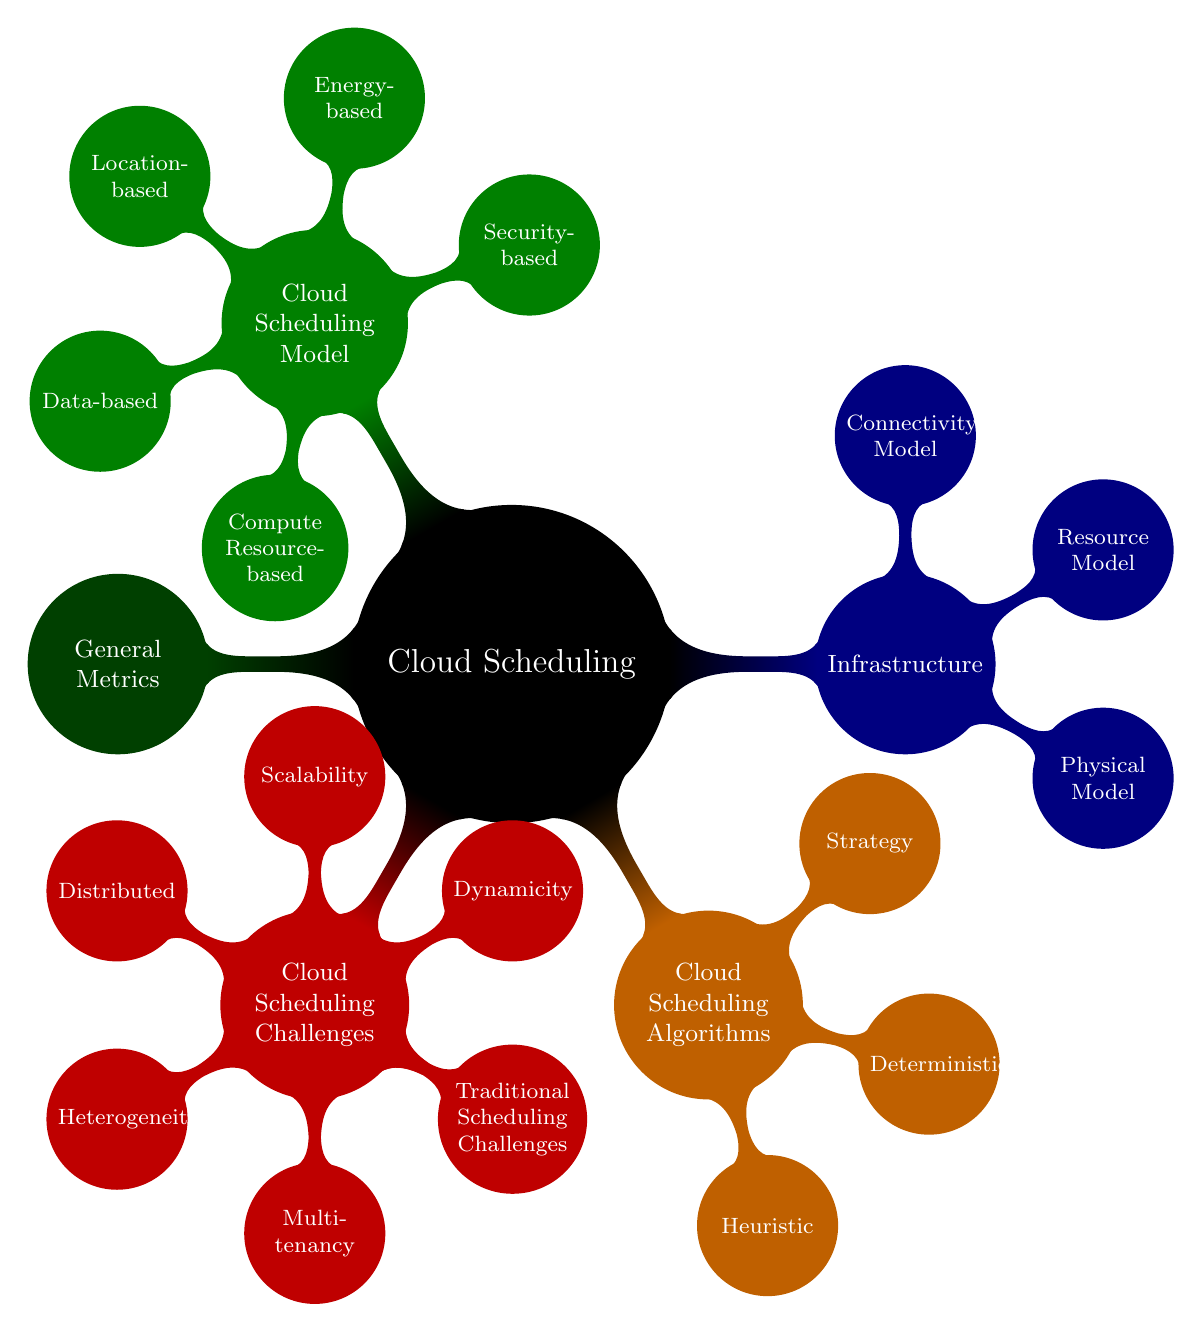
\begin{tikzpicture}
  \path[mindmap,concept color=black,text=white]
    
  node[concept] {Cloud Scheduling}
  [clockwise from=0]

  child[concept color=blue!50!black] {
      node[concept] {Infrastructure}
      [clockwise from=90]
      child { node[concept] {Connectivity Model} }
      child { node[concept] {Resource Model} }
      child { node[concept] {Physical Model} }
   }
  child[concept color=orange!75!black] {
      node[concept] {Cloud Scheduling Algorithms}
      [clockwise from=45]
      child { node[concept] {Strategy} }
      child { node[concept] {Deterministic} }
      child { node[concept] {Heuristic} }
   }
  child[concept color=red!75!black] {
      node[concept] {Cloud Scheduling Challenges}
      [clockwise from=-30]
      child { node[concept] {Diversity} }
      child { node[concept] {Multi-tenancy} }
      child { node[concept] {Heterogeneity} }
      child { node[concept] {Distributed} }
      child { node[concept] {Scalability} }
      child { node[concept] {Dynamicity} }
      child { node[concept] {Traditional Scheduling Challenges} }
  }
  child[concept color=green!25!black] {
      node[concept] {General Metrics}
  }
  child[concept color=green!50!black] {
      node[concept] {Cloud Scheduling Model}
      [clockwise from=-100]
      child { node[concept] {Compute Resource-based} }
      child { node[concept] {Data-based} }
      child { node[concept] {Location-based} }
      child { node[concept] {Energy-based} }
      child { node[concept] {Security-based} } 
   };
 \end{tikzpicture}
}
\end{figure}

\subsection{Resource Provider Focused Y-Cloud Taxonomy}\label{sec:y}

To showcase the interaction between the different layers more clearly
we like to refer the reader to the Y-cloud scheduling diagram
introduced by Laszewski in~\cite{lasbook}.

In this taxonomy we are concerned about how resources are placed on
physical models and are interconnected with each other to facilitate
scheduling algorithms. Figure~\ref{F:graph-y} depicts the different
models that are integral part of this taxonomy. It includes the 

\begin{description}

\item[Physical Model] representing major physical resource layers to
  enable a hierarchical scheduling strategy across multiple data
  centers, data centers, racks, servers, and computing cores.

\item[Resource Model] representing resource-based scheduling
  decisions while dealing with  containers and functions, virtual
  machines and jobs, virtual clusters, provider managed resources, and
  multi-region provider managed resources.

\item[Connectivity Model] introducing connectivity between components
  when addressing scheduling. This includes components such as memory,
  processes, connectivity to distributed resources, hyper-graphs to
  formulate hierarchies of provider based resources, and region
  enhanced hyper-graphs. The connectivity model allows us to leverage
  classical scheduling algorithms while applying such models and
  leveraging established or new scheduling algorithms for these
  models.

\end{description}

\begin{figure*}[p]
  \centering
  \resizebox{0.75\textwidth}{!}{%
  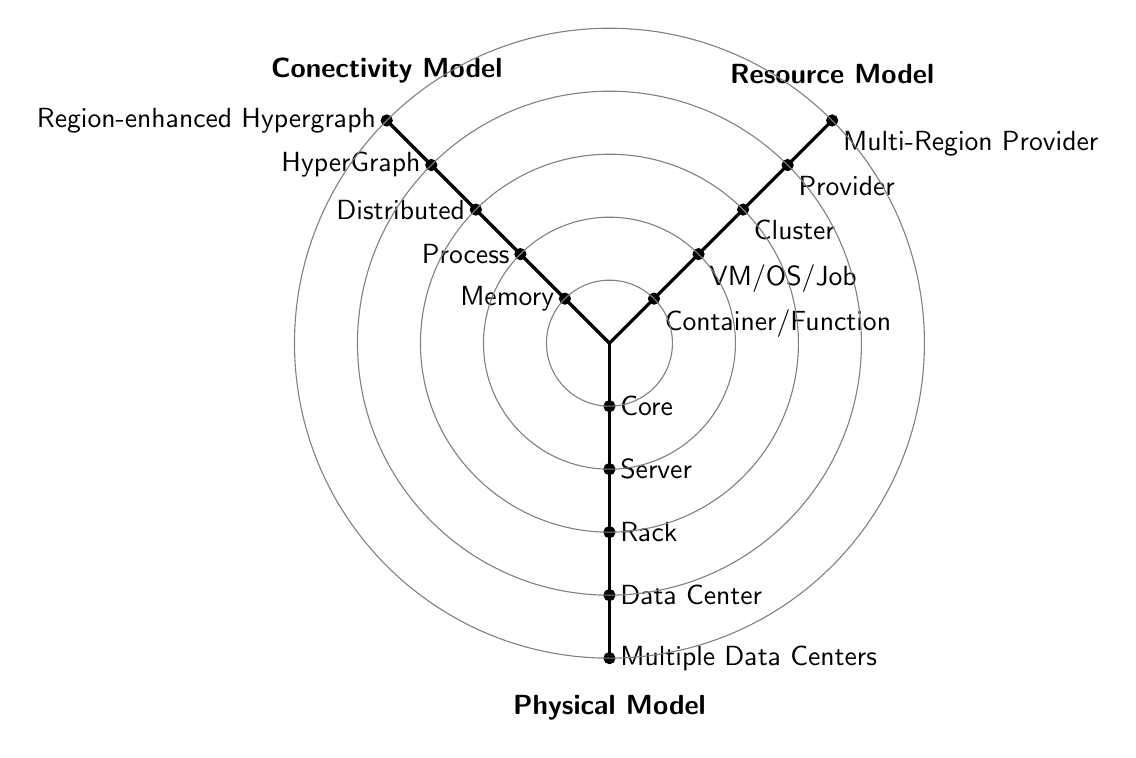
\begin{tikzpicture}[>=stealth',join=bevel,font=\sffamily,auto,on grid,decoration={markings,mark=at position .5 with \arrow{>}}]
  % \begin{tikzpicture}[>=stealth',join=bevel,font=\sffamily,auto,on grid,decoration={markings,mark=at position .5 with \arrow{>}}]
    %\input{y_chart_common}
    \coordinate (conectivityNode) at (135:4cm);
    \coordinate (resourceNode) at (45:4cm);
    \coordinate (physicalNode) at (270:4cm);
    \coordinate (originNode) at (0:0cm);

    \node [above=1em] at (conectivityNode) {\textbf{Conectivity Model}};
    \node [above=1em] at (resourceNode) {\textbf{Resource Model}};
    \node [below=1em] at (physicalNode) {\textbf{Physical Model}};

    \draw[-, very thick] (conectivityNode.south) -- (0,0) node[left,pos=0]{Region-enhanced Hypergraph} node[left,pos=0.2]{HyperGraph} node[left,pos=0.4]{Distributed} node[left,pos=0.6]{Process} node[left,pos=0.8]{Memory};

    \draw[-, very thick] (resourceNode.south) -- (0,0) node[pos=0]{Multi-Region Provider} node[pos=0.2]{Provider} node[pos=0.4]{Cluster} node[pos=0.6]{VM/OS/Job} node[pos=0.8]{Container/Function};

    \draw[-, very thick] (physicalNode.south) -- (0,0) node[right,pos=0]{Multiple Data Centers} node[right,pos=0.2]{Data Center} node[right,pos=0.4]{Rack} node[right,pos=0.6]{Server} node[right,pos=0.8]{Core};

    \draw[fill] (barycentric cs:conectivityNode=1.0,originNode=0) circle (2pt);
    \draw[fill] (barycentric cs:conectivityNode=0.8,originNode=0.2) circle (2pt);
    \draw[fill] (barycentric cs:conectivityNode=0.6,originNode=0.4) circle (2pt);
    \draw[fill] (barycentric cs:conectivityNode=0.4,originNode=0.6) circle (2pt);
    \draw[fill] (barycentric cs:conectivityNode=0.2,originNode=0.8) circle (2pt);

    \draw[fill] (barycentric cs:resourceNode=1.0,originNode=0) circle (2pt);
    \draw[fill] (barycentric cs:resourceNode=0.8,originNode=0.2) circle (2pt);
    \draw[fill] (barycentric cs:resourceNode=0.6,originNode=0.4) circle (2pt);
    \draw[fill] (barycentric cs:resourceNode=0.4,originNode=0.6) circle (2pt);
    \draw[fill] (barycentric cs:resourceNode=0.2,originNode=0.8) circle (2pt);

    \draw[fill] (barycentric cs:physicalNode=1.0,originNode=0) circle (2pt);
    \draw[fill] (barycentric cs:physicalNode=0.8,originNode=0.2) circle (2pt);
    \draw[fill] (barycentric cs:physicalNode=0.6,originNode=0.4) circle (2pt);
    \draw[fill] (barycentric cs:physicalNode=0.4,originNode=0.6) circle (2pt);
    \draw[fill] (barycentric cs:physicalNode=0.2,originNode=0.8) circle (2pt);

    \draw[black!50] (0,0) circle (4.0cm);
    \draw[black!50] (0,0) circle (3.2cm);
    \draw[black!50] (0,0) circle (2.4cm);
    \draw[black!50] (0,0) circle (1.6cm);
    \draw[black!50] (0,0) circle (0.8cm);
  \end{tikzpicture}
  }
  \caption{Resource Provider Focused Y-Cloud Taxonomy~\cite{las18cloudscheduling-whitepaper}.}
  \label{F:graph-y}
\end{figure*}


\subsection{Cloud Scheduling Model}

Now that we have identified the resource provider focused Y-Cloud
taxonomy we can identify some important classifications that govern the
scheduling decisions to effectively use these resources. This includes
metrics that influence the scheduling. Traditional scheduling metrics
and attributes for scheduling algorithms are shown in
Figure~\ref{F:graph-metrics}. They include typically cost, time, space,
reliability, energy, and security.


\begin{figure}[!th]
	\centering
\resizebox{0.6\columnwidth}{!}{%
\begin{forest}
skan tree
   [General Scheduling Metrics
        [Cost]
        [Time]
        [Space]
        [Reliability]
        [Energy]
        [Security]
   ]
]
\end{forest}
}
\caption{Traditional Compute Scheduling Metrics}
\label{F:graph-metrics}
\end{figure}


When looking into the specifics of these metrics applied to cloud
computing we can easily identify more details for these traditional
metrics that apply to the various infrastructure components that
constitute a cloud including compute, data, energy, quality of
service, and security. We depict some of the major attributes that
influence the scheduling decisions in Figure~\ref{F:graph-taxonomy}.
Furthermore each of the attributes in the categories Compute, Data,
Security, Energy, and Quality of service can be combined if not
already included in the specific scheduling attribute. For example in
order to identify scheduling model based on virtual machines,
attributes such as the once in data, energy, QoS, or security may be
introduced in the scheduling decision.



\begin{figure}[!th]
	\centering
\resizebox{\columnwidth}{!}{%
\begin{forest}
skan tree
[Cloud\\ Scheduling Model
   [Compute-Resource-based
     [Workflow-based]
     [Job-based]
     [VM-based
       [Migration]
       [Placement]
     ]
     [Task-based]
     [Container-based]
     [Function-based]
     [Platform-based]
   ]
   [Data-based
        [Storage Type]
        [Volume]
        [Redundancy]
        [Network-based
          [Bandwidth]
          [Latency]
        ]
    ]
    [Location-based
            [Processor-based]
            [Server-based]
            [Room-based]
            [Datacenter-based]
            [Region-based]
            [Global-based]
        ]  
    [Energy-aware
        [HVAC]
        [Green IT]
        [PUE]
        [Energy Source]
    ]
    [Security-based
        [Public]
        [Private]
    ]
   ]
]
\end{forest}
}
\caption{Cloud Scheduling Models}
\label{F:graph-taxonomy}
\end{figure}





This information can now be used to define provisioning and service
scheduling as categorized next.

\subsection{Taxonomy of Challenges in Cloud Scheduling}\label{sec:challange}

Some of the obvious cloud characteristics and challenges that lead to
a categorization are listed next and are summarized in
Figure~\ref{F:graph-challenges}.

\begin{description}

\item [Large scale:] Clouds offer large number of resources to its
  users that need to be optimally utilized under quality of service
  constraints set by providers and users. A cloud involving a plethora
  of resources spanning across the globe is obviously a huge
  infrastructure. The range of functions, tasks, jobs and applications
  need to be scheduled at any point of time onto available resources.
  Handling them in such scale requires efficient resource management.
  As such, scheduling becomes a complex endeavor, integrating dynamic
  and multi-faceted scheduling. 
            
\item [Dynamic nature of clouds:] Clouds encompass a dynamically
  changing resource environment of in which resources belong to
  different administrative domains keep on joining and leaving the
  clods. Hence scheduling must be adaptive and address the dynamic
  resource availability.

\item[Heterogeneous providers and services:] There is no single cloud.
  We have to recognize that the competitive nature in the cloud
  market promotes not only heterogeneous cloud providers, but also
  heterogeneous cloud services that may compete with each other and
  either offer the same or customized services targeting a particular
  user community. Resources in clouds are highly
  diversified in nature, capacity, working style and administrative
  domains. The inclusion of different resource providers with the
  desire to lock customers into their own services and products, makes
  heterogeneous multicloud scheduling multi-layered a formidable challange.

\item [Highly diversified:] Due to the large diverse set of
  applications (but also infrastructure) smart strategies to schedule
  such applications on the required resources are needed.

\item [Decentralized:] The resources in the cloud are distributed
  among various data centers, rack, and servers. Although they may
  belong to a provider, they can still be utilized across provider
  boundaries and even if within the same provider regions, calling for
  a high degree of decentralization.

\item[Limited control by users:] Due to the fundamental nature of the
  cloud access to low level scheduling mechanisms are often hidden and
  only available to the provider. On the other hand users still have
  their own scheduling requirements in regards to for example cost,
  and deadlines.
  
\item[Dynamic loads:] Due to the size of the user community sporadic
  burst on resource requirements lead to challenges to adjust
  provisioned resources and schedule application onto them.

\item[Security concerns:] Another important requirement for scheduling
  is the ability to integrate issues such as privacy and security
  considerations as the provider needs to assure that local laws as
  well as the general privacy and security concerns are addressed.
  This is especially of concern when government or health care
  providers need to schedule resources in a cloud for their
  application needs, making it necessary to distinguish problems that
  can be executed on public vs private clouds through scheduling but
  also through policy decisions that integrate with scheduling
  algorithms.
  
\end{description}

Thus we need to distinguish a number of scheduling challenges one of
which is governed by differentiating users and providers. Here, on
the one hand, we focus on cloud providers that try to utilize in the
best possible way the existing resources for the customers under
optimization constraints such as cost, high availability, fault
tolerance for the providing cloud resources and services. On the other
hand, we have customers that expect quality assurances, but also
have their own constraints such as deadlines, cost, and implicit
requirements from their applications including data placement and
management that may influence the scheduling decision,

In both cases we need to address the challenge of provisioning
resources and also the challenge of scheduling services onto these
resources. Although these steps can be done independently it is
obvious that interrelationship between them is needed in case of
re-provisioning and dynamic adaptation to dynamic loads placed on the
resources.

In both cases under-utilization prevents a resource from performing
optimally, incurring idle time, whereas over-utilization causes a
resource to degrade the node's performance.


\begin{figure}[htpb]
  \centering
  \resizebox{1.0\columnwidth}{!}{%
\begin{forest}
skan tree
   [Cloud Scheduling Challenges
        [Diversity
           [Infrastructure]
           [Platforms]
           [Services]
        ]
        [Multi-tenancy]
        [Heterogeneity]
        [Distributed]
        [Scalability
           [Huge Infrastructure]
        ]
        [Dynamicity]
        [Traditional Challenges
          [Efficiency]
          [Cost]
          [Time]
          [Space]
          [Reliability]
          [Energy]
          [Security
            [Authentication]
            [Authorization]
            [Auditing]
            [Privacy]
          ]
        ]
   ]
]
\end{forest}
}
   \caption{Scheduling challenges applied to all levels} 
  \label{F:graph-challenges}
\end{figure}




%%%%%%%%%%%%%%%%%%%%%%%%%%%%%%%%%%%%%%%%%%%%%%%%%%%%%%%%%%
\subsection{Taxonomy Classification of Resource Scheduling Algorithms}\label{S:algo}
%%%%%%%%%%%%%%%%%%%%%%%%%%%%%%%%%%%%%%%%%%%%%%%%%%%%%%%%%%

Next we present in Figure~\ref{F:graph-algorithm} a classification of
resource scheduling algorithms that we found while reviewing a
significant set of literature related to cloud computing. We focus in
Figure~\ref{F:graph-algorithm} on a relevant subset while focussing on
VM placement while considering QoS parameters to guide the scheduling
task. An additional classification is based on the type of algorithm
used for the scheduling task.  Dependent on the locality and large
scale of the scheduling task in many cases a deterministic approach is
not suitable. Hence, different algorithm categories are listed in
Figure~\ref{F:graph-scheduling}.

%When looking at heuristics~\cite{vivekanandan2011study}
%we find traditional algorithms such as hill-climbing but also a
%variety of nature inspired algorithms. The detail description of
%existing work in the field of resource scheduling algorithm is done in
%the next section.


\begin{figure}[!thbp]
	\centering
\resizebox{1.0\columnwidth}{!}{%
\begin{forest}
skan tree
[Resource Scheduling Algorithms
      [Strategy
        [Parallelism
          [Batch]
          [Asynchronous]
        ]
        [Cooperation
          [Co-operative]
          [Non-cooperative]
        ]
      ]
      [Deterministic]
      [Heuristic
            [Nature Inspired
              [Simulated Annealing]
              [Genetic Algorithms]
              [Ant Colony Optimization]
              [Particle Swarm Optimization]
            ]
            [Tabu Search]
            [Hill Climbing]
      ]
]
\end{forest}
}
\caption{A subset of Resource Scheduling Algorithms}
\label{F:graph-algorithm}
\end{figure}

\begin{figure}[!th]
	\centering
\resizebox{1.0\columnwidth}{!}{%
\begin{forest}
skan tree
[Resource Scheduling Algorithms
    [VM Placement-based 
        [Dynamic VM placement]
        [Network aware VM placement]
        [Energy aware VM placement]
    ]    
    [Quality of Service-based 
            [Cost-based]
            [Time-based]
            [Reliability-based]
            [Security-based]
    ]
    [Heuristic-based]
    [Container-based]
    [Function-based ]
]
\end{forest}
}
\caption{Classification of Resource Scheduling Algorithms}
\label{F:graph-scheduling}
\end{figure}


%%%%%%%%%%%%%%%%%%%%%%%%%%%%%%%%%%%%%%%%%%%%%%%%%%%%%%%%%%
%%%%%%%%%%%%%%%%%%%%%%%%%%%%%%%%%%%%%%%%%%%%%%%%%%%%%%%%%%
%%%%%%%%%%%%%%%%%%%%%%%%%%%%%%%%%%%%%%%%%%%%%%%%%%%%%%%%%%
%%%%%%%%%%%%%%%%%%%%%%%%%%%%%%%%%%%%%%%%%%%%%%%%%%%%%%%%%%
%%%%%%%%%%%%%%%%%%%%%%%%%%%%%%%%%%%%%%%%%%%%%%%%%%%%%%%%%%
%%%%%%%%%%%%%%%%%%%%%%%%%%%%%%%%%%%%%%%%%%%%%%%%%%%%%%%%%%



%%%%%%%%%%%%%%%%%%%%%%%%%%%%%%%%%%%%%%%%%%%%%%%%%%%%%%%%%%
\section{Literature review of Cloud Resource Scheduling Algorithms}\label{sec:literature}
%%%%%%%%%%%%%%%%%%%%%%%%%%%%%%%%%%%%%%%%%%%%%%%%%%%%%%%%%%

In this section we conduct an exemplary but extensive literature
review of cloud scheduling in order to confirm our {\bf taxonomy
  categories}. As part of this review, we present a number of tables
to identify the categories from research and frameworks we reviewed
and are related to cloud scheduling. We augmented each table with a
first column that is highlighted and refers to the cloud scheduling
taxonomy category we identified for this work.

To provide an additional guide while grouping some work together we
have introduced a number of sections focusing on a topic and grouped
the literature based on its main contribution into these
groups. However, we avoided double listing of the research in multiple
groups as much as possible to keep the tables small.

As a result we organize this section by scheduling categories related to 
%
dynamic scheduling (Section~\ref{sec:dynamic}),
cloud metric based scheduling with emphasize (Section~\ref{sec:vm-scheduling}) on 
energy (Section~\ref{sec:energy}),
network (Section~\ref{sec:network}),
cost (Section~\ref{sec:cost}),
time (Section~\ref{sec:time}),
reliability (Section~\ref{sec:reliability}),
security (Section~\ref{sec:security}), 
and heuristics (Section~\ref{sec:heuristic}).

As High Performance Computing in the cloud is also a service offered
by several providers, w also review scheduling for HPC in the cloud
(Section~\ref{sec:hpc}) and scientific workflows
(Section~\ref{sec:workflow}) which is going to become a field of
interest for the scientific community as the transition to clouds
takes place and is explicitly an area of interrest fro NIST as
discussed in the Big Data Reference Architecture Working Group while
leveraging activities from the community including the past Grid
community.

In this sections we also review papers with emphasize on scheduling in
public clouds (Section~\ref{sec:public}), 
containers (Section~\ref{sec:container}), function as a service
(Section~\ref{sec:faas}) as well as distributed resource providers
(Section~\ref{sec:distributed}) which can utilize a service mesh
(Section~\ref{sec:mesh}).





\subsection{Dynamic Scheduling}\label{sec:dynamic}



As part of this scheduling task we often also find the distinction
between static scheduling, where resources are scheduled once and dynamic scheduling, which is
constantly updated during execution to find better resource
utilization over time. The later is often motivated by need for
scalability~\cite{keller2014hierarchical} across and within data
centers or increased fault
tolerance~\cite{tighe2013distributed}. Association of other metrics
into the dynamic scheduling approach is common to for example
integrate power, reduce network bandwidth and enable more
sophisticated Service level agreements~\cite{tighe2013distributed}. In
many cases not only the cloud user, but obviously also the cloud
provider can benefit from dynamic
scheduling~\cite{tighe2014integrating}. We find that it can be
beneficial to separate the scheduling task in multiple steps such as
shown in~\cite{sun2015live}. Here live migration for correlated VMs is
optimizing on data, compute, and bandwidth. Other cloud metrics such
as price~\cite{tordsson2012cloud} are also common and will be in more
detail addressed in Section ~\ref{sec:cost}. Obviously a rich number
of algorithm can be applied such as shown in
Section~\ref{sec:heuristic}.

Table~\ref{T:dynamic-scheduling} lists a number of efforts related to
dynamic scheduling while focusing on virtual machine placement.


\newcolumntype{g}{>{\columncolor{Gray}}p}
\begin{table*}[!htbp]
 \caption{Comparison of Dynamic Scheduling Algorithms}
     \label{T:dynamic-scheduling}
   \centering
\scriptsize
\resizebox{\textwidth}{!}{%
\begin{tabular}{|g{2cm} p{2cm} p{2cm} p{2cm} p{2cm} p{2cm} p{2cm} p{1.5cm}|}
  \hline
 \textbf{Taxonomy Classification} & \textbf{Author} & \textbf{Basis} & \textbf{Advantages} & \textbf{Disadvantages} & \textbf{scheduling techniques} & \textbf{Experimental Scale} &\textbf{Experimental Parameters}

\\ \hline

 Energy-basedd, energy source & Sun et al.~\cite{sun2015live} & Introduction of a virtual data center to solve VM migration issues & Low complexity & Fixed band-with & Heuristic algorithm & Simulated environment & VM migration cost and time
\\ \hline

Energy-basedd, VM migration & Tighe et al.~\cite{tighe2014integrating} & Auto scaling  algorithm  alongside  a  dynamic VM  allocation  algorithm  & Reduce a number of migrations & No optimization criteria &Rule based heuristic&  DCSim & Power, SLA, Migrations 
\\ \hline

Energy-based & Keller et al.~\cite{keller2014hierarchical} &  Management of data center resources to reduce the management scope &  Reducing  the  overhead  in  the  data centre management network & High complexity & Greedy algorithm & DCSim  & Power, number of migrations, average number of racks, active hosts 
\\ \hline 

Energy-based, PUE & Tighe et al.~\cite{tighe2013distributed} &  Trade-off  among number of  migrations, SLA  violation and power & Consider energy and SLA & more bandwidth usage & First fit algorithm &  DCSim  & Power consumption, number of migrations, SLA violations 
\\ \hline 

Compute-resource based, VM based & Tordsson et al.~\cite{tordsson2012cloud} &  Optimized placement of applications in multi-cloud environments & Emphasized on Price and performance in terms of hardware configuration, load balancing & Ignored security and energy efficiency at time of scheduling & Integer programming formulations & Amazon EC2 & Throughput, number of jobs 
\\ \hline


Energy-based, VM-based & Younge et al.~\cite{las10cloudsched} & 
Power aware & 
reduces cost & 
slight reduction in performance & 
heuristic & on premise cloud & 
power consumption 

\\ \hline

\end{tabular}
}
\end{table*}




\subsection{Cloud Metric-based Scheduling}\label{sec:vm-scheduling}

Due to the complexity of cloud environments, many different metrics
are used to guide the scheduling of virtual machines, containers,
platforms, tasks, batch jobs and workflows. As already pointed out
many different metrics that influence their schedule (see
Figure~\ref{F:graph-metrics}).

% Figure ~\ref{F:graph-metrics-flower} showcases
%
\begin{figure}[phtb]
  \centering
  \resizebox{0.5\columnwidth}{!}{%
\smartdiagram[bubble diagram]{Scheduling Metrics, Cost, Time, Security, Energy, Reliability}
}
   \caption{Multi-phase scheduling in a hierarchical resource model} 
  \label{F:metrics}
\end{figure}

\subsubsection{Energy Aware Scheduling}\label{sec:energy}



Energy consumption is a key issue for cloud providers due to the
enormous cost associated with operating large cloud data center. By
using server consolidation, optimizing operation on physical machines
and using dynamic voltage scaling processors, energy consumption can
be reduced as shown in~\cite{las09dvfs,las10dvfs,calheiros2014energy}.

Various scheduling methods such as minimize the total
makespan~\cite{bessis2013using}, dynamic
meta-heuristic~\cite{bi2017application}, fractal
mathematics~\cite{duan2016energy}, and machine learning clustering and
stochastic~\cite{bui2017energy} have been utilized.


It is obvious that multiple metrics must be included the correlate for
example CPU, RAM and bandwidth~\cite{zhu2017three}. Dynamicity, for
example, while addressing peak loads~\cite{duan2016energy} or
migration~\cite{beloglazov2010energy} has naturally also an impact on
the energy cost. Energy in hybrid and multiple data centers in the
clouds is used
in~\cite{quarati2013hybrid,garg2011environment,gai2016dynamic} while
at the same time increasing the cloud provider brokers revenue. Energy
consumption in heterogeneous clouds has also been
considered~\cite{ding2015energy}.  Others create models to predict the
energy consumption of each virtual machine~\cite{kim2014energy} this
requires certainly proper monitoring of the underlying server farms in
the cloud in~\cite{van2012comparison}. Integration of historical or
previous program executions while recording their energy consumption
can also be utilized~\cite{hu2010scheduling}. Others focus on
predicting future resource consumption needs~\cite{dabbagh2015energy}.






A comparison of energy aware scheduling algorithm in cloud computing is shown in
Table~\ref{T:g}.



\begin{sidewaystable*}[!htbp]

\caption{Comparison of Energy-aware VM Placement-based Scheduling
  Algorithms (A)}\label{T:g-a}
 \hspace{8pt}
\centering
\scriptsize
\resizebox{\textwidth}{!}{%
\begin{tabular}{|g{2.1cm} p{1.5cm} p{2cm} p{2cm} p{2cm} p{2cm} p{2cm} p{2cm}|}
  \hline
  % after \\: \hline or \cline{col1-col2} \cline{col3-col4} ...
\textbf{Classification} & \textbf{Author} & \textbf{Basis} & \textbf{Advantages} & \textbf{Disadvantages} & \textbf{scheduling techniques} & \textbf{Experimental Scale} &\textbf{Experimental Parameters} 
\\ \hline

  \makecell{Energy source, \\Compute\\ resource-based, \\Job-based} & Calheiros et al.~\cite{calheiros2014energy} & Intelligent scheduling combined DVFS capability  &  Improved energy efficiency  & Ignored Network and Storage energy consumption  &  Rank method   & Cloud Sim & Energy consumption
\\ \hline 

\makecell{Energy-aware, \\PUE} & Bessis et al.~\cite{bessis2013using} & Improving communication for Distributed systems at the time of scheduling & Improved system performance & High complexity & Graph theory concepts & SIMIC & makespan, latency times 
\\ \hline 
  
\makecell{Energy-aware,\\ Energy source, \\Cost, \\VM-based} & Bi et al.~\cite{bi2017application} & Dynamic Scheduling algorithm for reducing energy consumption & Focused on performance and energy cost & High complexity due to virtualized Data centers & meta heuristic methods & Simulated environment & Profit, CPU utilization  
\\ \hline   

    \makecell{Energy-aware,\\ Compute\\ resource-based, \\VM-based} & Duan et al.~\cite{duan2016energy} & Scheduling of VM machines & Improved the CPU load prediction & No optimization & Ant colony optimization &  CloudSim & Energy Consumption
\\  \hline 

  \makecell{Energy-aware,\\ Energy source,\\ Cost, \\VM-based} & Bui  et al.~\cite{bui2017energy} & Balance between energy efficiency and quality of service & Low complexity & Ignored cost, scalability & Greedy first fit algorithm & Simulated Environment & Energy, Memory, CPU  
\\ \hline


\makecell{Energy-aware,\\ Energy source, \\ Cost,\\ VM-based} & Zhu et al.~\cite{zhu2017three} & Data center balance while saving power consumption & Improved management of VM resource & High complexity &  Multi-dimensional vector bin packing problem-based heuristic & CloudSim & SLA violations, Resource utilization
\\ \hline

\makecell{Energy-aware, \\ Energy source,\\ VM-based} & Beloglazov et al.~\cite{beloglazov2010energy} &  Enhancement of resource utilization by re-allocation of the resources. & Considered different types of workloads, No prior information about applications & Ignored cost and time & Heuristic algorithm & CloudSim & Energy, Average SLA, migrations
  \\ \hline

  
\makecell{Energy source,\\ Compute\\ resource-based , \\VM-based}  & Quarati et al.~\cite{quarati2013hybrid} &  Reservation of a quota of private resources & Reduced energy consumption and carbon emission & Lacks implementation on a real-world cloud platform & Round robin algorithm & Discrete Event Simulator & User satisfaction, energy saving, energy consumption
\\ \hline

  \makecell{PUE, \\ Job-based} & Garg et al.~\cite{garg2011environment} &  Optimal scheduling policies & Reduced energy cost, energy consumption & Ignored security & Meta-scheduling policies & Simulated environment  & Average energy consumption, average carbon emission, arrival rate of application
 \\ \hline
 

\end{tabular}
}
\end{sidewaystable*}
  

 \begin{sidewaystable*}[!htbp]

   \caption{Comparison of Energy-aware VM Placement-based Scheduling Algorithms (B)}\label{T:g-b}
   \hspace{8pt}
  
\centering
\scriptsize
\resizebox{\textwidth}{!}{%
\begin{tabular}{|g{2cm} p{1.5cm} p{2cm} p{2cm} p{2cm} p{2cm} p{2cm} p{2cm}|}
  \hline
  % after \\: \hline or \cline{col1-col2} \cline{col3-col4} ...
\textbf{Classification} & \textbf{Author} & \textbf{Basis} & \textbf{Advantages} & \textbf{Disadvantages} & \textbf{scheduling techniques} & \textbf{Experimental Scale} &\textbf{Experimental Parameters} 
   
\\ \hline

\makecell{Energy-aware,\\ VM-based} & Keke et al.~\cite{gai2016dynamic} & Cloudlets for energy reduction & Reduced energy consumption & No time consideration & FCFS scheduling policy & DECM-Sim & Energy consumption 
\\ \hline
  
\makecell{Energy source,\\ VM-based} & Dabbagh et al.~\cite{dabbagh2015energy} &  Energy-aware resource management decisions  & improved performance & No optimization criteria, high complexity& K-means clustering& Testbed & Average CPU and Network utilization
\\ \hline

    \makecell{Energy source, \\VM-based} & Kim et al.~\cite{kim2014energy} & VM energy consumption estimation model & Reduced cost, power consumption & More complex to implement, Ignored time & Power aware scheduling algorithm & Xen 4.0 hypervisor & Energy consumption, error rate
\\ \hline

\makecell{Compute\\ resource-based,\\ VM-based} & Van Do et al. in~\cite{van2012comparison} & Interaction aspects between on-demand requests and the allocation of virtual machines & Reduced energy consumption & No cost and time optimization & Power aware scheduling algorithm & Numerical Simulation & Average Energy consumption, average heat emission
\\ \hline

  
  \makecell{Energy-aware,\\ Energy source, \\Compute \\resource-based, \\
  VM-based (migration),\\ Workflow} & Li et al.~\cite{li2016energy} & Scheduling algorithm to reduce energy consumption while meeting the deadline constraint & Focused on energy consumption & Ignored  processing power energy consumption, VM migration & Heuristic method & Simulated environment & Energy consumption
\\ \hline 


  \makecell{Energy source,\\PUE, \\ VM-based} & Ding  et al.~\cite{ding2015energy} & Dynamic VMs scheduling & Increased Processing Capacity & Ignored VM migration, Power penalties of status transitions of processor & FCFS & Simulated environment  & Deadline, Energy consumption 
\\ \hline 



\end{tabular}
}
\end{sidewaystable*}


\subsubsection{Network Aware Scheduling}\label{sec:network}




As clouds project remote large scale resources network traffic to,
from, and within must be considered for scheduling. This not only
contains moving data in and out of the compute center or storage, but
also may contain message exchange between to sometime complex
distributed applications that run in these cloud data
centers. Minimizing the distance between data providers and data
consumers while for example replicating data~\cite{www-akamai} can save
significant amount of traffic and has long been applied in the
internet as one of its beneficial strategies. Service level agreements
(SLA)~\cite{breitgand2012improving} are playing an important role to
achieve proper utilization as part of the scheduling effort. Treating
the network as shared scarce resource~\cite{rampersaud2016sharing}
motivates the development of network-based scheduling algorithms.
Just as in other metric-based scheduling models, we find the
distinction between static~\cite{biran2012stable} and dynamic
scheduling during runtime so we can deal with traffic bursts.

A variety of resource abstractions (see Figure~\ref{F:class-metric}) are
applicable also to scheduling as part of the network traffic, such as
demonstrated by~\cite{yu2017survivable} to optimize traffic in virtual
clusters.  Scheduling across on multiple layers is especially of
benefit for networking~\cite{bi2015sla} to minimize across different
tiers.  Scheduling of platforms such as Hadoop offers naturally
advantages when networking is integrated~\cite{kondikoppa2012network}.  Having access to lower level infrastructure
such as offered by OpenStack presents opportunities to include Network
Function Virtualization (NVF)~\cite{lucrezia2015introducing}

Table \ref{T:c} shows examples for network aware scheduling algorithms
in cloud computing.



  \begin{sidewaystable*}[p]
\caption{Comparison of Network-aware VM Placement-based Scheduling Algorithms}\label{T:c}
\centering
\scriptsize
\resizebox{\textwidth}{!}{%
\begin{tabular}{|g{2cm} p{2cm} p{2cm} p{2cm} p{2cm} p{2cm} p{2cm} p{1.9cm}|}
  \hline
   \textbf{Classification} & \textbf{Author} & \textbf{Basis} & \textbf{Advantages} & \textbf{Disadvantages} & \textbf{scheduling techniques} & \textbf{Experimental Scale} &\textbf{Experimental Parameters} 
   
\\ \hline

VM based & Yu et al.~\cite{yu2017survivable} & Service provisioning on IaaS platform while focusing on the inter-connected
VMs. &  High availability & High complexity & Heuristic algorithm & Simulator & Average VM consumption ratio, average running time 
\\ \hline 

Compute resource based, VM based & Bi et al.~\cite{bi2015sla}~\cite{bi2016trs} & Architecture for self management of data centers & Considered temporal request of multi-tier web applications  & does not consider security parameters  & Queuing approach &  trace-driven simulation & Cost 
\\ \hline

 Compute resource based & Rampersaud et al.~\cite{rampersaud2016sharing} & Used page-sharing concept to handle VM Packing problem & Improvement of memory sharing during allocation decisions & High complexity & Linear programming technique & Simulated environment & Memory reduction, number of excess servers 
\\ \hline

 Compute resource-VM based & Lucrezia et al.~\cite{lucrezia2015introducing} & Investigated OpenStack for the deployment of network service graphs & Increased throughput & Analyzing time is more, Ignored policy-constraints in  order  to  define  administration  rules&  Brute force algorithm  & KVM hypervisors &  VM locations, traffic throughput and latency 
\\ \hline 

Compute resource VM based & Biran et al.~\cite{biran2012stable}& Consideration of traffic  bursts  in  deployed  services & Minimizing  the  maximum load  ratio  over  all  the  network & Ignored energy consumption& Greedy heuristic algorithm & Testbed & Average packet delivery delay , placement solving time  
\\ \hline




Compute-resource based workflow based & Kondikoppa et al.~\cite {kondikoppa2012network} & To make Hadoop scheduler aware of network topology & Improved data locality& Ignored cost, energy, security & FIFO &Eucalyptus  based testbed & Execution time, delay for scheduling task 


\\ \hline

\end{tabular}
}
\end{sidewaystable*}



\subsubsection{Cost Aware Scheduling}\label{sec:cost}


Cost in clouds arise for using the data center facilities. These costs
are passed along to the users. Through shared use of the facilities
and keeping under-utilization low, clouds can have an advantageous
cost performance in regards to on-premise compute and data
centers. Costs for such centers include hardware operation cost such
as energy and equipment, as well as, operating costs such as software
licensing and update and personnel costs. Dependent on the hardware
and software used, cloud providers offer a tiered cost model that
allows users to assess need for data, speed, and reliability as part
of their cost.  Other options such as renewable energy use of the data
center in case of energy aware customers may also play a role.

Cost aware scheduling has been applied to virtual
machines~\cite{yuan2017ttsa},
tasks~\cite{yuan2017temporal,zuo2015multi},
workflows~\cite{arabnejad2015cost,arabnejad2016budget}, as well as
high-throughput~\cite{yuan2016cawsac} computing.  Revenue
maximization~\cite{yuan2018warm} has not only been applied to metrics
such as latency~\cite{ghahramani2017toward}, but is also useful via
advanced dynamic Voltage and Frequency Scaling
(DVFS)~\cite{las10cloudsched,calheiros2014energy} due do reducing the
high energy costs with little performance reduction. This also could
be achieved through delayed execution~\cite{bi2016trs} or relaxation
of deadlines~\cite{zhang2018dynamic}.  Other strategies include the
introduction of penalties as part of SLA~\cite{wu2012sla}. Typical
resource utilization such as optimizing processor
sharing~\cite{lee2012profit} data placements~\cite{lee2012profit},
have known to decrease cost. Obviously also dynamic
adaptations at run-time allow reduction of cost~\cite{ari2013design}

Table \ref{T:e} presents a comparison of cost aware scheduling algorithms.



%\begin{sidewaystable*}[p]
\begin{table}[htb]
\caption{Comparison of Cost-based Scheduling Algorithms}\label{T:e}
\hspace{8pt}
\centering
\scriptsize
\resizebox{\textwidth}{!}{%
\begin{tabular}{|g{2cm} p{2cm} p{2cm} p{2cm} p{2cm} p{2cm} p{2cm} p{1.9cm}|}
  \hline
   \textbf{Classification} & \textbf{Author} & \textbf{Basis} & \textbf{Advantages} & \textbf{Disadvantages} & \textbf{scheduling techniques} & \textbf{Experimental Scale} &\textbf{Experimental Parameters} 

\\ \hline                                                                                                                                                                              
                                                                                                                                                                              
  \makecell{Compute\\ resource-based,\\ Task-based,\\ Cost-based} & Bi et al.~\cite{bi2015sla}~\cite{bi2016trs} & Architecture for self management of data centers & Considered temporal request of multi-tier web applications  & does not consider security parameters  & Queuing approach &  trace-driven simulation & Cost
  \\ \hline
  
\makecell{Compute\\ resource-based,\\  data-based,\\  task,\\  Latency,\\  VM-based,\\ Cost-based} & Yuan et al.~\cite{yuan2017ttsa,yuan2017temporal} & Emphasizing profit maximization & handles service delay bound & High complexity  & PSO and SA & simulation environment & Revenue
\\ \hline

\makecell{Compute\\ resource-based,\\  Task-based,\\ Cost-based}  & Zuo et al.~\cite{zuo2015multi} & Multi-objective Task Scheduling  & Improved  performance & Ignored energy consumption & Ant colony optimization & CloudSim & Cost, makespan, deadline violation rate
\\ \hline

\makecell{Compute\\ resource-based,\\  Workflow-based,\\ Cost-based} & Arabnejad et al.~\cite{arabnejad2015cost} &  Re-use of pre-provisioned instances for scheduling & Less complexity& Ignored security and energy efficiency& Deadline early Tree algorithm & CloudSim & Cost and deadline
\\ \hline

\makecell{Compute\\ resource-based,\\ VM-based,\\ Cost-based} & Wu et al.~\cite{wu2012sla} &  VM usage efficiency designed utility function by considering dynamic VM deploying time, processing time and data transfer time & Improved cost saving & Does not support security and energy efficient  & Admission control and scheduling algorithm & CloudSim & Average response time, total profit
\\ \hline

\makecell{Data-based,\\ Cost-based} & Lee et al.~\cite{lee2012profit} &  Personalized
features of the user request and the elasticity of SLA properties & Reduced operational costs and increase profits & Objectives conflict with each other & binary integer programming & CloudSim & Average utilization, average net profit rate, average response time  
  \\ \hline


\makecell{Compute\\ resource-based,\\  VM-based,\\ Cost-based} & Ari et al.~\cite{ari2013design} &  Finite Element Analysis cloud service with a focus on mechanical structural analysis, performance characterization and job scheduling issues & Throughput improvement and resource utilization & Ignored cost& Adaptive algorithm & Testbed & Throughput and time
\\ \hline

  
\end{tabular}
}
\end{table}
%\end{sidewaystable*}


\subsubsection{Time based Scheduling}\label{sec:time}



Cloud users have the desire to reduce the time it takes to execute
their applications. This is often motivated to fulfill
deadlines~\cite{arabnejad2017scheduling}.

Besides virtual machine and task scheduling it is also important to
integrate data-aware scheduling to reduce access time to the
data~\cite{vandenbosshe2013}.

\TODO{THIS REFERNCE DOES NOT EXIST}

\TODO{Reference is in table too}

As already mentioned previously, historical
data~\cite{thomas2015credit} or proxies~~\cite{erdil2013autonomic}
about execution times help designing time-aware scheduling algorithms.

We find algorithms that integrate
deadline constraint ~\cite{li2016energy}, 
completion time~\cite{xu2011job} with fairness,
low downtime to improve time for execution~\cite{frincu2014scheduling},
and 
delay bounds 
~\cite{yuan2017time}.

Table~\ref{T:f} presents a comparison of time aware
scheduling algorithms.

\begin{sidewaystable*}[!htbp]
   \caption{Comparison of Time-based Scheduling Algorithms}
    \label{T:f}
\centering
\scriptsize
\resizebox{\textwidth}{!}{%
\begin{tabular}{|g{2cm} p{1.9cm} p{2cm} p{2cm} p{2cm} p{2cm} p{2cm} p{2cm}|}
  \hline
  % after \\: \hline or \cline{col1-col2} \cline{col3-col4} ...
 \textbf{Classification} & \textbf{Author} & \textbf{Basis} & \textbf{Advantages} & \textbf{Disadvantages} & \textbf{scheduling techniques} & \textbf{Experimental Scale} & \textbf{Experimental Parameters} 
 
\\ \hline

Compute-resource based, task & Yuan et al.~\cite{yuan2017time} & Task scheduling in green data centers & Investigated temporal variations &  Ignored energy consumption and cost & PSO and SA & Simulated Environment & Delay bound and time 
\\ \hline

 Compute resource based workflow & Arabnejad et al.~\cite{arabnejad2017scheduling} & Dynamically provisioned commercial cloud environments & Evaluation of task selection algorithms reveals impact of workflow symmetry & High complexity & Rank method & CloudSim & Response time, Cost 
\\ \hline

Compute-resource based, Workflow & Thomas et al.~\cite{thomas2015credit} & Task length aware scheduling & Lesser makespan and increased resource utilization & No comparison with existing algorithm & Min-min & CloudSim & Makespan 
\\ \hline 

Compute-resource based, VM & Frincu~\cite{frincu2014scheduling} & A priory scheduling and  searching for an optimal allocation of components on nodes in order to ensure a homogeneous spread of component types on every node. & Minimizing the application cost & Centralized approach represents a single point of failure & Nonlinear-programming & Simulator platform & Average load per node, optimal allocation, reliability 
\\ \hline

Compute-resource based, VM & Erdil~\cite{erdil2013autonomic} & Disseminated information as agents of dissemination sources for resource scheduling & Availability of resource state, reduces dissemination overhead & Ignored cost as parameters & Adaptive proxy algorithm & Scalable simulation network framework & Query satisfaction rates, random walk hop count limit 
\\ \hline


 Compute-resource based, Data based, Task-based & Van den Bossche et al. in~\cite{vandenbosshe2013} & Deadline-based workloads in a hybrid cloud setting & Minimize cost and time & does not handle multiple workflows & hybrid scheduling approach & Simulator & Total Cost, application deadline met, turnaround time, data transferred 
\\ \hline

Compute-resource based , task & Xu et al.~\cite{xu2011job} & Berger model and assign tasks on optimal resources to meet user's QoS requirements & Optimal completion time & Ignored cost and energy efficiency, security& Resource allocation algorithm and then followed by job scheduling & CloudSim & Time, bandwidth 
\\ \hline


\end{tabular}
}
\end{sidewaystable*}


\subsubsection{Reliability Aware Scheduling}\label{sec:reliability}



Users and providers need the guarantee of reliability. Thus many
scheduling efforts integrate how to increase reliability. Strategies
such as replication of data and compute services are common
practice. Obviously this comes often at a price and increased cost may
occur when reliability is concerned. The distributed nature of clouds
make it a formidable challenge to offer reliability. However at the
same time while providing large scale data centers to offer cloud
services with highly specialized operating staff and abilities to
replicate and migrate workloads to other services increases
reliability when compared to on-premise data centers due to larger
efficiency of the cloud data centers in regards to overall cost for
its users.

Various studies have been conducted to analyze the effect of reliability on clouds.

This includes reliability assessment models
~\cite{malik2012reliability}, integration of communication and
networks~\cite{jing2015reliability}, increase of resource
availability~\cite{latiff2016fault}. Trade offs between different
scheduling metrics such as energy and reliability have also been
studied~\cite{tang2016energy}.

A comparison of reliability and scheduling is given in Table~\ref{T:h}.



\begin{sidewaystable*}[!htbp]
\caption{Comparison of Reliability-based Scheduling Algorithms}\label{T:h}
\hspace{8pt}
\centering
\scriptsize
\resizebox{\textwidth}{!}{%
\begin{tabular}{|g{2cm} p{2cm} p{2cm} p{2cm} p{2cm} p{2cm} p{2cm} p{1.9cm}|}
  \hline
   \textbf{Classification} & \textbf{Author} & \textbf{Basis} & \textbf{Advantages} & \textbf{Disadvantages} & \textbf{scheduling techniques} & \textbf{Experimental Scale} &\textbf{Experimental Parameters} 
\\ \hline

\makecell{Compute\\ resource-based,\\ Job-based,\\ Reliability-based} & Malik et al.~\cite{malik2012reliability} & Reliability assessment mechanism for scheduling resources & Reliability assessment algorithms for general applications and real time applications  & No security and energy parameters consideration & Max -min & Amazon EC2 cloud & Fault tolerance, time
\\ \hline

\makecell{Compute\\ resource-based,\\ Job-based,\\ Reliability-based} & Jing et al.~\cite{jing2015reliability} &  Model for fault-tolerant aware scheduling &  Low complexity  & No cost, time optimization & Adaptive secure scheduling algorithm & Simulated environment & Reliability
\\ \hline
  
\makecell{Compute\\ resource-based,\\ Task-based,\\ Reliability-based} & Abdulhamid et al.~\cite{latiff2016fault} & Uncountable numeric nodes for resource in clouds & Lower makespan & No optimization & League championship algorithm & CloudSim & Failure ratio, the failure slowdown and the performance improvement rate
\\ \hline

\makecell{Energy-aware ,\\ Energy source,\\ Reliability-based} & Tang et al.~\cite{tang2016energy} &  Reliability and energy-aware task scheduling architecture & To get good trade off among performance, reliability, and energy consumption & No support for cost optimization& Heuristic method & Discrete event simulation environment  & Schedule length, Energy consumption,  Application reliability 
 \\ \hline


\end{tabular}
}
\end{sidewaystable*}


\subsubsection{Security based Scheduling}\label{sec:security}



As mentioned earlier security as a key issue cloud users and
providers require in order for cloud infrastructure to be useful for
many applications.

Virtual machine scheduling requires the need for isolation, that can
be controlled by security
policies~\cite{afoulki2011security}. Isolation can also apply to the
incoming and outgoing data~\cite{chejerla2017qos,kashyap2014security}.
Risks occurring by inspecting the connections among VMs
~\cite{shetty2016security} can be analyzed and integrated in
scheduling strategies.  To enable trust between components in the
cloud background key exchanges have been proposed~\cite{liu2013ccbke}
Multi-objectives (possibly contradictory) need to be also
considered. Most often it includes cost vs. security scheduling
frameworks~\cite{kashyap2014security,zeng2015saba,wang2012cloud}.  As
many edge devices need to interface with cloud services due to their
computational and data limitations, privacy-preserving solutions to
interface between clouds and mobile devices have been considered
~\cite{bilogrevic2011meetings}.

Security based scheduling algorithms are presented (see
Table~\ref{T:i}). 



\newcolumntype{g}{>{\columncolor{Gray}}p}
\begin{table*}[!htbp]
\caption{Comparison of Security based Scheduling Algorithms}
     \label{T:i}
\centering
\scriptsize
\resizebox{\textwidth}{!}{%
\begin{tabular}{|g{2cm} p{2cm} p{2cm} p{2cm} p{2cm} p{2cm} p{2cm} p{1.9cm}|}
  \hline
  \textbf{Taxonomy Classification} & \textbf{Author} & \textbf{Basis} & \textbf{Advantages} & \textbf{Disadvantages} & \textbf{scheduling techniques} & \textbf{Experimental Scale} & \textbf{Experimental Parameters} 

\\ \hline

Compute-resource and Data based  & Chejerla et al.~\cite{chejerla2017qos} &  Scheduling of resources in cloud integrated Cyber-physical Systems & Consideration of security, time & High complexity &Heuristic algorithm & Simulated environment & Speed up, resource utilization, makespan 
\\ \hline

Compute-resource based, VM based & Shetty et al.~\cite{shetty2016security}& VM placement techniques to reduce security risks & Reduced computing costs and deployment costs& No optimization criteria & Heuristic algorithm& Simulated environment & Cost, security risks & 
\\ \hline 

Compute resource based-workflow & Zeng et al.~\cite{zeng2015saba} & Scheduling algorithm for resource utilization & Low complexity & Ignored energy consumption & Clustering and prioritization algorithm  &  Simulated environment & Makespan and speed up 
\\ \hline 

Compute-resource based, VM based & Kashyap et al.~\cite{kashyap2014security}& Secure aware scheduling of real time based applications & Improved response time and overall security & High complexity & Priority Algorithm & Hypervisor & Deadline, Security 
\\ \hline 

Compute-resource based, Workflow & Liu et al.~\cite{liu2013ccbke} &  Scheme for security aware scheduling &  Reduced the computational load and execution time  & No cost optimization involved & Adaptive secure scheduling algorithm & KVM hyper-visor & Time unit consumed per computational load 
\\ \hline

Compute-resource based, Task based & Wang et al.~\cite{wang2012cloud} & Uncountable numeric nodes for resource in clouds& Provided scheduling of resources in secure way & Ignored cost & Bayesian  algorithm& CloudSim & Trust value, average schedule length 
\\ \hline

Compute-resource based, VM based & Afoulki et al.~\cite{afoulki2011security}& Security risk management in a cloud &  Less complexity & Consolidation issues while implementing policies & Greedy Algorithm & Simulated environment & VM placement time  
\\ \hline 

Compute-resource based, VM based & Bilogrevic et al.~\cite{bilogrevic2011meetings} & Scheduling services on the cloud for mobile devices & Enhanced Performance & No support cost optimization, Ignores power consumption by the network & Privacy aware scheduling schema & Testbed & Time, Data exchanged, privacy in approach 
 \\ \hline
\end{tabular}
}
%\tiny}

\end{table*}


\subsection{Heuristic based Scheduling}\label{sec:heuristic}



Heuristic methods help to design efficient algorithm to fulfill the
users application requirements. We provide here a small sample of
different heuristics as found in literature. This includes particle
swarm optimization~\cite{pandey2010particle}, multi-objective genetic
algorithm-based ~\cite{mezmaz2011parallel,gkasior2016metaheuristic},
colony optimization with swarm intelligence~\cite{mateos2013aco}, bee
colony~\cite{ld2013honey}, artificial neural
networks~\cite{kousiouris2011effects}, simulated
annealing~\cite{torabzadeh2010cloud},
game-theory~\cite{gkasior2016metaheuristic}, and Game theory by
minimizing the Pareto dominance and makespan~\cite{su2013cost}.  Other
heuristics utilize classical models such as using the critical path in
multi-phase scheduling algorithms ~\cite
{abrishami2013deadline}. Besides virtual machines we often also find
workflows to be the scheduling unit in
heuristics~\cite{bousselmi2016qos}.

A comparison of heuristic methods based scheduling
algorithm is done in~\ref{T:j}.



\begin{sidewaystable*}[!htbp]
\caption{Comparison of Heuristic-based Scheduling Algorithms}\label{T:j}
\centering
\scriptsize
\resizebox{\textwidth}{!}{%
\begin{tabular}{|g{2cm} p{2cm} p{2cm} p{2cm} p{2cm} p{2cm} p{2cm} p{2cm}|}
  \hline
  % after \\: \hline or \cline{col1-col2} \cline{col3-col4} ...
 \textbf{Classification} & \textbf{Author} & \textbf{Basis} & \textbf{Advantages} & \textbf{Disadvantages} & \textbf{scheduling techniques} & \textbf{Experimental Scale} &\textbf{Experimental Parameters} 
   

\\ \hline

Compute resource based, job based & Gasior et al.~\cite{gkasior2016metaheuristic} & Parallel and distributed scheme  for  scheduling  jobs  & Multi-objective optimization, consideration of security risks also& No cost consideration & Genetic algorithm & Simulation Testbed & Flow time, makespan, turnaround time 
\\ \hline


Compute resource based, workflow based & Bousselm et al.~\cite{bousselmi2016qos} & QoS based & Consideration of QoS parameters & High complexity & Parallel Cat Swarm Optimization& Simulated environment  & Execution time, execution and storage cost, availability of resources and data transmission time 
\\ \hline

Compute resource based, job based & Cristian et al.~\cite{mateos2013aco} & Scheduler for job scheduling, consider static cloud  & Minimize weighted flowtime and makespan & does not handle energy consumption & Ant colony optimization and swarm intelligence approach & CloudSim & makepan 
\\ \hline

Compute resource based, workflow & Abrishami et al.~\cite{abrishami2013deadline} & Cost-optimized,  deadline-constrained execution of workflows in cloud. considered required run-time and data estimates in order to optimize workflow execution & Minimize execution cost with in deadline & Ignored data transfer time, security & PCP algorithm & Simulated environment & Normalized cost 
\\ \hline

Compute resource based, task based & Sen et al.~\cite{su2013cost} & Cost-efficient task-scheduling algorithm using two heuristic strategies & Reduced monetary costs & Ignored security & Heuristic strategies & Numerical experiments & Makespan 
\\ \hline

 Compute-resource based, Job based & Gutierrez-Garcia et al.~\cite{gutierrez2013family} & Scheduling of Bag-of-tasks based on allocation times of virtualized cloud resources & Makespan & Ignored cost & Heuristic algorithm &  Testbed & Makepan, overhead time
\\ \hline

Compute resource based, task based, energy based & Babu~\cite{ld2013honey} & Based  priority of tasks, designed load balancing algorithm & Maximize throughput & High operational complexity & Honey Bee algorithm & CloudSim & Makespan, Number of task migrations 
\\ \hline

Compute resource based, task based & Kousiouris et al.~\cite{kousiouris2011effects}& Virtual machines affect the performance of other VMs executing on the same node & Reduce performance overhead & Lacks implementation on a real-world cloud platform  & Genetic algorithm  &  Simulated environment & Degradation, test score delay 
\\ \hline

Compute resource based, Job based & Mezmaz et al.~\cite{mezmaz2011parallel} & Addressed the precedence-constrained parallel applications for cloud computing & Reduced energy consumption & High complexity of implementation and operation& Genetic algorithm & Simulated environment & Energy, speed up 
\\ \hline


Compute resource based, VM based & Torabzadeh et al.~\cite{torabzadeh2010cloud} & Flowshow job problem  & Minimized makespan and mean completion time & Not considered cost & Simulated annealing & Simulated environment & Computation time 
\\ \hline


\end{tabular}
}

\end{sidewaystable*}



\subsection{AI based Scheduling}\label{sec:AI}

\color{red}

Deep Reinforcement Learning (DeepRL) based approaches can
automatically learn to schedule more efficiently and can also adapt to
any system changes. AI based approached can be used to handle the
scheduling decisions in Cloud computing environment. Various studies
have been conducted to analyze the effect of AI based scheduling
approach in the Cloud computing environment. This includes deep
reinforcement approach ~\cite{cheng2018drl,mao2018learning},
Q-learning model~\cite{zhang2017energy} and Q network model
~\cite{wang2019multi}. Markov decision based approach
~\cite{barrett2013applying} is also studied to handle the uncertainty
to provide optimal decision at the tiem of scheduling.  A comparison
of artificial intelligence based scheduling algorithm is done
in~\ref{T:j1}.

\color{black}
\begin{sidewaystable*}[!htbp]
\caption{Comparison of ML-based Scheduling Algorithms}\label{T:j1}
 \hspace{8pt}
\centering
\scriptsize
\resizebox{\textwidth}{!}{%
\begin{tabular}{|g{2cm} p{2cm} p{2cm} p{2cm} p{2cm} p{2cm} p{2cm} p{2cm}|}
  \hline
  % after \\: \hline or \cline{col1-col2} \cline{col3-col4} ...
 \textbf{Classification} & \textbf{Author} & \textbf{Basis} & \textbf{Advantages} & \textbf{Disadvantages} & \textbf{scheduling techniques} & \textbf{Experimental Scale} &\textbf{Experimental Parameters}


\\ \hline

\makecell{Compute \\resource-based,\\ Job-based,\\ ML-based} & Mingxi Cheng et al.~\cite{cheng2018drl} &  Two stage resource provisioning and/or task scheduling processor & Consideration of energy consumption aspects & No security consideration  & Reinforcement approach & Simulation Testbed & Energy cost and runtime
\\ \hline


\makecell{Compute \\resource-based,\\ Workflow-based,\\ ML-based} & Hongzi Mao et al. ~\cite{mao2018learning} & Presented Decima scheduler & Consideration of low latency scheduling decisions & High complexity & Reinforcement learning method & Simulated environment  & Execution time
\\ \hline

\makecell{Compute \\resource-based,\\ Job-based,\\ ML-based} & Qingchen Zhang et al. ~\cite{zhang2017energy} & A hybrid dynamic voltage and frequency scaling (DVFS) scheduling algorithm   & Minimize energy consumption & does not handle security & Deep Q-learning model & Simulation environment & energy consumption
\\ \hline

\makecell{Compute \\resource-based,\\ Workflow-based,\\ ML-based} & Yuandou Wang et al. ~\cite{wang2019multi} & Focused on workflow scheduling & Minimize energy consumption & Ignored time, security & Markov method & Simulated environment & Energy efficiency
\\ \hline

\makecell{Compute \\resource-based,\\ Task-based,\\ ML-based} & Enda Barret et al. ~\cite{barrett2013applying} & Guided  an optimal decision in the process of resource allocation & Reduced Time & Ignored security & Deep Q learning method & Simulation & Makespan
\\ \hline


\end{tabular}
}

\end{sidewaystable*}

%%%%%%%%%%%%%%%%%%%%%%%%%%%%%%%%%%%%%%%%%%%%
% HPC AND CLOUD
%%%%%%%%%%%%%%%%%%%%%%%%%%%%%%%%%%%%%%%%%%%%


\subsection{HPC and Cloud Computing Scheduling}
\label{sec:hpc}


Next we review scheduling classifications related to traditional High
Performance Computing (HPC). It is important to recognize, that HPC
and its frameworks must not be excluded as part of cloud scheduling
due to its exposure for scientific application in industry and
academia. More importantly HPC is now also offered as one of the supported
compute services in public cloud providers. When looking at the services offered
and needed we distinguish HPC batch queuing in the cloud, cloud
bursting of on premise HPC tasks, container isolation, on demand
platforms and bare metal provisioning.

\begin{description}

\item[HPC Batch Queuing in the Cloud.] These are specialized
  high-performance super-computing systems that are offered to
  customers with computation needs that can only be fulfilled by large
  scale specialized hardware. Grand challenge problems are often
  motivators for such hardware. In industry we for example find
  computational fluid dynamics, and modeling of biochemical processes
  as one of its user communities. Example offerings for HPC in AWS
  \cite{www-aws-hpc}, Azure~\cite{www-azure-hpc}, Google~\cite{www-google-hpc},
  but also other less prominent clouds such as Penguin Computing HPC
  in the cloud~\cite{PODHPCCloud2019}, and
  SabalCore~\cite{Sabalcore2019}.
  
\item[Cloud Bursting of On Premise HPC tasks.] The HPC systems are
  often over-utilized and thus the situation of resource starvation is
  to be considered. For this reason many batch queuing system allow
  the integration of cloud resources in such a fashion that task and
  workflows may be executed in the cloud through the integration of
  commercial or on premise cloud resources. In this case the term
  cloud bursting is used
  \cite{CloudBursting2019,BurstingHPC2019}. Example for the
  integration in prominent HPC scheduling includes
  Slurm~\cite{www-slurm}, Univa Grid Engine~\cite{www-univa},
  PBSpro~\cite{www-pbs-manual}, LSF~\cite{www-lsf},
  Moab~\cite{www-moab}.

  \color{red}
  Table ~\ref{T:l} present the comparison of the different batch resource management systems.
  
  \color{black}

\item[Container Isolation.] Due to the usage of queuing systems it is
  also possible to provide in part an improved container security
  framework, while executing containerized tasks as part of the
  queuing system. An example would be to utilize all cores in a
  compute server that is allocated with a queuing system
  processor. This feature can be integrated into many queuing systems
  while using Singularity~\cite{www-singularity}.

\item[On Demand Platforms.] Resource starvation in academic cloud and
  super computing centers motivate also the ability to run platforms
  that would typically run also in the cloud but provide a cheaper
  alternative if run locally in the existing HPC centers. A good
  example is Hadoop that can be run through
  myhadoop~\cite{krishnan2011myhadoop} in HPC centers~\cite{SDSC2019}.

\item[Bare Metal Provisioning.] In other cases it may be better to
  provide bare metal provisioning capabilities in case the
  existing platform or cloud abstraction may not be sufficient.
  Academic efforts such as FutureGrid~\cite{fox2013futuregrid} now
  followed by Comet~\cite{las-comet} and Chameleon Cloud~\cite{Chameleoncloud2019} 
  are good examples for it. Commercial
  efforts in this regard include OpenStack Ironic
 ~\cite{OpenstackIronic2019}, IBM~\cite{IBMBareMetal2019}, AWS
 ~\cite{AWS2019} and Rackspace~\cite{Rackspace2019}.

\end{description}


\begin{sidewaystable*}[p]

  % \centering
\caption{Comparison of Different Batch Resource Management Systems}\label{T:l}
\hspace{8pt}
\centering
\scriptsize
\resizebox{\textwidth}{!}{%
\begin{tabular}{|g{2cm} p{1.9cm} p{2.3cm} p{2cm} p{1.5cm} p{2cm}|}
  \hline
 \textbf{Classifaction} &   
 \textbf{Framework} & \textbf{Batch Features} &  \textbf{Cloud Bursting} & \textbf{Containers} & \textbf{Comment}  
\\ \hline

\makecell{Cloud bursting,\\ Cluster model} & Slurm~\cite{www-slurm} & 
Policy driven, backfill, exclusive and non-exclusive access to compute nodes & 
AWS, Azure, Google, Oracle & 
Yes & 
Open Source, popular
  \\ \hline

\makecell{Cloud bursting,\\ Cluster model} & Univa Grid Engine~\cite{www-univa} & 
Policy driven, backfill, exclusive and non-exclusive access to compute nodes, fault tolerant master & 
AWS, Azure, Google & 
Yes & 
previously SUN Grid Engine, Genias Codine
\\ \hline  
  
\makecell{Cloud bursting,\\ Cluster model} & Load Sharing Facility (LSF)~\cite{www-lsf} & 
Policy driven, backfill, exclusive, non-exclusive access to compute nodes &  IBM Cloud, AWS, Google and Azure & 
Yes & 
Previously OpenLava, IBM  Open Source 
\\ \hline

\makecell{Cloud bursting,\\ Cluster model} & Moab~\cite{www-moab} & 
Fairness policies, dynamic priorities, and extensive reservations &
AWS, Azure, Oracle, Google &
Yes & 
Open Source
\\ \hline
  
\makecell{Cloud bursting,\\ Cluster model} & Open Portable Batch System (OpenPBS)~\cite{Openpbs2018,Henderson1995} & 
Policy driven, backfill, exclusive and non-exclusive access to compute nodes, fault tolerant master & 
AWS, Azure, Google, Oracle & 
Yes & 
Open Source
\\ \hline



\end{tabular}
}

\end{sidewaystable*}



%%%%%%%%%%%%%%%%%%%%%%%%%%%%%%%%%%%%%%%%%%%%
% WORkflow
%%%%%%%%%%%%%%%%%%%%%%%%%%%%%%%%%%%%%%%%%%%%


\subsection{Workflow Scheduling Frameworks} 
\label{sec:workflow}



In the previous sections we already pointed out several workflow
related scheduling algorithms while using specific metrics to conduct
the scheduling. In addition we can integrate virtual machines,
containers, and tasks. The main intent of the cloud workflow is to automate
repeated task in a reliable way. 


Traditionally, workflow schedulers are often distinguished by
DAG~\cite{deelman2005pegasus,deelman2004pegasus,thain2005distributed}
and non-DAG scheduling while some support
both~\cite{las-karajan,las-cogkit-1,las06-workflow-book}.
For cloud workflow management services such as
Nintex ~\cite{www-nintex-wf}, Amazon Simple Workflow,
Hadoop streaming ~\cite{www-hadoop-streaming} for
map reduce workflows are used. The main intent of Amazon
simple workflow is to provide the support to build,
run, and scale background jobs that have parallel or
sequential steps The main intent of Spark
streaming ~\cite{www-spark-streaming} is to provide scalable,
high-throughput and fault-tolerant
stream processing of live data streams. Argo ~\cite{www-argo-wf},
a container-native workflow
engine is used for orchestrating parallel jobs on Kubernetes.

 Even prior
to the official FaaS frameworks existed that focused on the execution
of functions~\cite{las-infogram}.  Scientific applications such as
bio-informatics have introduced not only workflow systems, but also
promoted graphical workflow design tools to create dependency graphs
the are executed by workflow
schedulers~\cite{oinn2004taverna,tan2010comparison}.
  
In addition to our findings, in~\cite{yu2005taxonomy} workflows are
also organized by design, scheduling and data movement abilities.

It is often an overlooked fact that existing HPC batch queuing systems
contain features for job dependency management. In many cases these
features can be used to accommodate the users needs for scheduling
workflows onto the same hardware or in some cases clusters that are
managed through the same queuing
system
~\cite{www-lsf,www-moab,www-univa-GE-manual,www-pbs-manual}.







\subsection{Scheduling in Public Cloud Providers}
\label{sec:public}



Next, we compare scheduling methods and needs offered in public cloud
service providers are presented. This includes AWS, Azure, Google,
Rackspace, but also academic clouds such as FutureGrid and
FutureSystems Comet, Jetstream, and Chameleon Cloud.

It is important to recognize that today public cloud providers offer
not only virtual machines to the users, but a large variety of
compute, data, and analytical services. Some of them may even use bare
metal while others are having heightened security demands to for
example fulfill heath care or government isolation needs as part of
the infrastructure. All these issues naturally influence the
scheduling efforts which need to be addressed by the provider. In many
cases we do not find some of the information on how such scheduling is
conducted due to security and company secrets.

However we find metrics that users can utilize to formulate their own
strategies as we have introduced in the previous section if such
metrics are communicated to the users. This typically includes cost
and allows to leverage for example virtual machine with reliability
constraints such as AWS spot pricing compared to regular
pricing~\cite{AmazonEC22015}.  Cost also motivates users to suspend
usage of VMs instead of running them without concern. This has
happened to the authors of this paper, where in a class a student,
refused to shutdown experimental virtual machines and within two weeks
consumed thousands of compute hours on an academic cloud, while the
actual calculation was irrelevant.

One of the schedulers provided by public clouds are job and instance
schedulers that promote start and stop times for the resources
used~\cite{AWSIns2019,AzureSch2019,Rackspace2016,GoogleAppEngine2018}. Such
schedulers can integrate functions, data and compute instances. More
sophisticated schedulers can switch workloads between cloud data
centers~\cite{MicrosoftAzure2014}.

In ~\cite{Rackspace2016} cloud load-balancer, round robin and least
connections based algorithms are commonly used so that workload could
be distributed equally on all resources.  As one of the original tasks
of clouds was hosting of Web services under traffic load. public
clouds include strategies the scale up and down the services based on
such loads and allocate dynamically through a scheduler resources to
fulfill this demand.

Other providers have focused on making use of multi-cloud virtual
machine placement possible while offering optimization strategies for
workflows~\cite{CloudSigma2016} including detailed analysis of cost
metrics~\cite{Cloudmetrics2019}

Other efforts such as~\cite{las12fg-bookchapter,fox2013futuregrid}
have early on uniquely focused on scheduling bare metal resources
between the use of HPC and clouds, while running HPC queuing systems
on the same resources as cloud resources. Dynamic provisioning allowed
resources to be provisioned to the one or the other by
demand. In~\cite{las-comet} the re-provisioning is even done with the
help of a traditional batch queuing system.

Table~\ref{T:iaas} depicts examples as used in public cloud providers.



\begin{sidewaystable*}[!htbp]
\caption{Comparison of Different IaaS Models}\label{T:iaas}
\centering
\scriptsize
\resizebox{\textwidth}{!}{%
\begin{tabular}{|g{2cm} p{1.9cm} p{2cm} p{1.0cm} p{2cm} p{1.9cm} p{1.9cm} p{2cm}|}
  \hline

  \textbf{Classification} & 
\textbf{Provider or Framework} & \textbf{Pricing} &  
\textbf{Database RDS} & \textbf{Reliability} & \textbf{Monitoring} & 
\textbf{Base OS}   & \textbf{Programming Framework}
 \\ \hline
 
& Amazon EC2~\cite{AmazonEC22015} & Pay-as-you-go or Yearly, reserved, spot & My SQL, Ms SQL, Oracle & Good & Good & Linux and windows & Python, Java, PHP, Ruby 
\\ \hline

& Microsoft Window Azure~\cite{MicrosoftAzure2014} &  Pay-as-you-go, semester, year &  Microsoft SQL Database & Average & Average & Windows and linux & Java, Php, .net 
\\ \hline

& Rackspace~\cite{Rackspace2016} &  Pay-as-you-go  & MySQL & Good & Extensive  & Ubuntu & Java, Python 
\\ \hline

& Google App Engine~\cite{GoogleAppEngine2018} & Pay as you go & Cloud SQL & Extensive & good & linux, free BSD, windows & Python,  Java,  PHP and Go, Node.js
\\ \hline

& Cloud Sigma~\cite{CloudSigma2016} & Pay-as-you-go  & SQL & Good& Good & Average &Python, Java, PHP, Python, Ruby, Clojour 
\\ \hline

%Openstack~\cite{Openstack2018} & Pay-as you go, monthly  & My SQL& Good & Extensive & Linux, windows & Python, Perl, PHP,  
%\\ \hline
%\textbf{Digital Occean} & Pay-as-you-go or Monthly, semester, year  &100\%  & 5 & Poor & None & Python, Perl, PHP 
%\\ \hline
%Open Nebula~\cite{OpenNebula2018} &Subscription &My SQL  & High & Good & Linux & C,C++, Ruby, java, 
%\\ \hline

& Future Grid (discontinued)~\cite{las12fg-bookchapter,fox2013futuregrid} & Free Academic &  User Choice &  Good & Good &  Linux & Openstack, OpenCirrus, Eucalyptus, Cloudmesh
  \\ \hline
  
& Chameleon Cloud~\cite{las-chameleon} & Free Academic &  User Choice &  Moderate & Moderate &  Linux & Openstack
  \\ \hline
\end{tabular}
}
\end{sidewaystable*}



\subsection{Scheduling in Container Frameworks}
\label{sec:container}


Container schedulers provide mechanisms to fine-tune the selection
processes of containers onto distributed
resources~\cite{Containers2018,de2018distributed}. Typically a default
scheduling policy is provided. Policies might place new services on
hosts with the fewest currently active services.

Based on our Y-diagram we need to distinguish 2 different
services. First, scheduling on the same server and second scheduling
on a number of servers that are treated typically as one abstract
resource.

For the first scheduling task we need to consider data management to
efficiently utilize the memory hierarchy, but also for example
execution deadlines or privacy concerns to organize the computation
tasks as required. In the distributed case we also need to integrate
communication related issues. We focus next on the distributed
frameworks in more detail we focus on Docker Swarm, Kubernetes,
Singularity, and Mesos.

\begin{description}


\item[Docker Swarm.] Docker Swarm is a clustering and scheduling
tool for Docker containers~\cite{Dockerswarmengine2018} across compute
servers. In a docker swarm we distinguish manager nodes and worker
nodes. The manager uses load balancing to place the containers onto
the worker nodes. Once a task is placed on a server it is executed
there.  Docker swarm uses a single scheduling
strategy~\cite{Dockerswarm2018}.



\item[Kubernetes.] Kubernetes is an open-source orchestrator
developed by Google for automating container management and
deployment~\cite{Kubernates2018}. The basic deploy-able object is a
Pod which consists of one or more containers running in a shared
context. An API is used to declare policies and scalability
constraints. The Kubernetes scheduler is topology aware and workload
aware which can be integrated into the policy policy constraints to
expose availability, performance and capacity. Auto-scaling, load
balancing and secrets managements are also provided by Kubernetes.

\item[Singularity.] Singularity can be using a variety of
container frameworks as backend. It allows the use of containers
without being superuser. Due to this, singularity is a popular choice
for running containers on traditional HPC
systems~\cite{www-singularity}. Due to this scheduling can be
supported directly by the under-laying queuing system.


\item[Mesos.] Mesos~\cite{hindman2011mesos,Mesos2018} provides an
API for resource management and scheduling in data centers. Mesos
abstracts CPU, memory, storage, and other compute resources. It
integrates fault-tolerance. Mesos provides a thin resource sharing
layer that helps to furnish fine-grained sharing by providing common
interfaces among different cluster frameworks. It's goal is improved
utilization, respond quickly to workload changes, by maintaining
system's capability in terms of scalability and robustness.


\item[Community Efforts.] Many community efforts to improve
container scheduling are conducted. This includes for example the use
of genetic algorithm~\cite{guerrero2018genetic}, container and host
selection policies for cloud deployment models~\cite{hanafy2017novel}
with SLA's, the characterization of
applications~\cite{medel2017client} scheduling of virtual
clusters~\cite{dziurzanskivalue}, and migration~\cite{Flocker2018},
and systems integrating multiple schedulers such as Nomad which offer
service scheduler, batch scheduler and a systems scheduler while
focusing on the support of long running jobs~\cite{Nomad2018}.
\end{description}
Table ~\ref{T:z} shows the comparison of existing work related to scheduling. 




%\begin{sidewaystable*}[!htbp]
\begin{table*}[htb]
\caption{Comparison of Container-based Scheduling Algorithms}\label{T:z}
\hspace{8pt}
\centering
\scriptsize
\resizebox{\textwidth}{!}{%
\begin{tabular}{|g{2cm} p{2cm} p{2cm} p{2cm} p{2cm} p{2cm} p{2cm} p{2cm}|}
  \hline
 
\textbf{Classification} & \textbf{Author} & \textbf{Basis} & \textbf{Advantages} & \textbf{Disadvantages} & \textbf{scheduling techniques} & \textbf{Experimental Scale} &\textbf{Experimental Parameters}

\\ \hline

\makecell{Compute\\ resource-based,\\ Container-based} & Guerrero et al.~\cite{guerrero2018genetic} &   Optimize physical machine utilization & Increase resource utilization & High complexity & Genetic Algorithm & Simulation environment & Resource Utilization , Performance
\\ \hline

  \makecell{Compute\\ resource-based,\\ Energy-aware,\\ Container-based} & Hanaf et al.~\cite{hanafy2017novel} &  Container and host selection policies & Improved SLA & Highly complex & Pre-Selection method & Simulated environment & Energy Consumption
\\ \hline


\makecell{Compute\\ resource-based,\\ Container-based} & Medel et al.~\cite{medel2017client} & Scheduler for minimizing resource contentions & Reduce resource contention & Ignored Time optimization & Priority algorithm & Kubernetes &  Time
\\ \hline

\makecell{Compute\\ resource-based,\\ Container-based} & Dziurzanski et al. \cite{dziurzanskivalue} & Optimization of the container allocation & Easy to implement & Ignored network optimization & Heuristic method & Simulated environment & Performance
\\ \hline

\makecell{Compute\\ resource-based,\\ Container-based} & Guerrero et al. \cite{guerrero2018resource} & Optimized the deployment of micro services-based applications & Improved security & High complexity & Genetic algorithm & Simulation environment & Resource utilization
\\ \hline


\end{tabular}
}
%\tiny}

\end{table*}
%\end{sidewaystable*}








\subsection{Function Scheduling Algorithms}
\label{sec:faas}



To further improve scheduling on cloud resources, the concept of
function as a services was introduced.  It allows the invocation of
small functions with limited resource constraints on
servers~\cite{lasbook}. For example a minimum execution time per
request is five minutes provided by AWS lambda and azure
functions~\cite{ServerlessComputing2018}. It supports manage user
defined functions on highly available infrastructure in an unified
manner~\cite{nastic2017serverless}. This also allows the scheduling of
workflows comprised out of
functions~\cite{alqaryouti2018serverless}. In~\cite{fox2017status} we
discuss the status of serverless computing and function as a service
in Industry and research.  Serverless computing is considered the
backend for running FaaS at runtime. System allocation and other
resource management activities are provided by the backend. Thus the
users has not to worry about activities conducted by the
server. Hence, the name serverless computing. Through the use of FaaS
and serverless computing cost can be reduced by more efficiently
scheduling smaller tasks on resources.

A number of FaaS frameworks exist that can be used on public clouds
but also self hosted clouds or network of workstations.

Scheduling in FaaS is provided by triggers. Such triggers offer a
publish subscribe model in which events are conducted, once the
trigger is fired. This includes triggers for time, data, and
executions. Time based scheduling is supported by cron.  These
frameworks are supported by all major public clouds including AWS
lambda~\cite{AWSlambda2018}, Google cloud
functions~\cite{GoogleCF2018}, Azure Function~\cite{Azure2018}

Other open source frameworks such as Apache
OpenWhisk~\cite{OpenWhisk2018} allow users to install FaaS services on
their own infrastructure.


\subsection{Scheduling among Distributed Resources and Providers}
\label{sec:distributed}





Users may have the desire to not only use services on one cloud but on
multiple clouds. This is motivated largely by avoiding vendor lock-in,
unique service offerings, or combining services from different
vendors.

%\begin{sidewaystable*}[p]
\begin{table}[htb]
%\centering
\caption{Comparison of other Resource Management Systems}\label{T:distr-cloud}
\hspace{8pt}
\centering
\scriptsize
\resizebox{\textwidth}{!}{%
\begin{tabular}{|g{2cm} p{1.9cm} p{2cm} p{2cm} p{2cm} p{2cm} p{2cm} p{2cm}|}
  \hline
\textbf{Classification} &
  \textbf{Framework} & \textbf{Architecture} &  \textbf{Usage} & \textbf{Open source} & \textbf{Support} & \textbf{Applications}   & \textbf{Programming Framework} 
\\ \hline

\makecell{Datacenter-based} & Eagle~\cite{delgado2016job} & Hybrid & Differentiates short and long jobs & EPFL IC IINFCOM LABOS, Switzerland & Spark & Different workloads and Parallel jobs & Python, Java, PHP, Python, Ruby 
\\ \hline

\makecell{Cluster-based} & Hopper~\cite{ren2015hopper} &  Decentralized &  Speculation-aware job scheduler & Microsoft Research & Spark  & CPU intensive & Java, Php, .net
\\ \hline

\makecell{Cluster-based} & Tetris~\cite{grandl2015multi} & Centralized & Multi-resource bin-packing & Microsoft & Generic applications & CPU intensive & Python, Perl, Java, PHP, Ruby, Node.js, Erlang, Scala
\\ \hline

\makecell{PaaS-based,\\ Data-based} & Fawkes~\cite{ghit2014balanced} & Centralized & Dynamic resource balancing &TU Delft & Mapreduce frameworks & Data intensive & Python, Java, PHP, Python, Ruby 
\\ \hline

\makecell{Cluster-based} & Omega~\cite{schwarzkopf2013omega} &  Decentralized & Shared state abstraction & University of Cambridge & Custom applications & Parallel applications &Java, Php, .net
\\ \hline

\makecell{Peer-to-Peer} & OurGrid~\cite{andrade2003ourgrid} & Centralized  & Equitable Resource Sharing & Universidade Federal de CampinaGrand, Brazil & Generic applications  & Bag of Tasks  & Java, Python
\\ \hline

\makecell{PaaS-based,\\ Data-based} & Sparrow~\cite{ousterhout2013sparrow}& Decentralized & Randomized sampling approach &  U.C. Berkeley AMPLab & Spark& CPU intensive& Python, Perl, Java, PHP, Ruby, Node.js, Erlang, Scala, Clojure, .Net
\\ \hline

\makecell{PaaS-based,\\ Data-based} & Yarn~\cite{vavilapalli2013apache} & Monolithic  & Resource requests with containers &Hadoop  & Spark & Data intensive  &Python, Java, PHP, Python, Ruby, Clojour
\\ \hline

%Mesos~\cite{Mesos2018} & Two way protocol  & Pessimistic resource offers & University of California, Berkeley & Spark & CPU and Data Intensive & Python, Perl, PHP, Rest, Ruby, .net, C\#
%\\ \hline

\end{tabular}
}
\end{table}

%\end{sidewaystable*}



Such efforts contain Eagle, a hybrid data center scheduler for
data-parallel programs~\cite{delgado2016job};
Hopper~\cite{ren2015hopper}, a job scheduler that trades off existing
and speculated job scheduling decisions; Tetris
~\cite{grandl2015multi}, a cluster scheduler that aims to match
multi-resource task requirements with resource availability;
Fawkes~\cite{ghit2014balanced} a multi-cluster systems for map-reduce;
Omega~\cite{schwarzkopf2013omega} with optimistic concurrency control;
OurGrid~\cite{andrade2003ourgrid,cirne2006labs} for worldwide
computing platform with isolated environments;
Sparrow~\cite{ousterhout2013sparrow} and fine-grained task scheduling
scheduler.
  
We can also find more prominent schedulers such a contains Apache's
  Hadoop YARN~\cite{vavilapalli2013apache} which acts as a resource
  management systems to for example schedule Hadoop distributed
  processing framework considering QoS, scalability, higher efficiency
  and fair resource usage.

We contrast different resource management systems, used for
maintaining resources in distributed environments such as Clouds (see
Table \label{T:distr-cloud}).

\subsection{Service Mashups} 
\label{sec:mesh}

To support scheduling across clouds and services, service mashups can
be used. This includes long standing efforts such as Cloudmesh, which
targets the creation of reproducible environments to easily manage
virtual machines, bare metal provisioned operating systems, platform
deployments and more recently data services in a multi-cloud
environment. It is a goal to integrate custom schedulers in such
service mashups. Another example is Terraform~\cite{www-terraform}
which focuses on reproducible environments.




%%%%%%%%%%%%%%%%%%%%%%%%%%
%%%%%%%%%%%%%%%%%%%%%%%%%%
%%%%%%%%%%%%%%%%%%%%%%%%%%
%%%%%%%%%%%%%%%%%%%%%%%%%%
%%%%%%%%%%%%%%%%%%%%%%%%%%


\section{Conclusion and Lessons Learned}\label{sec:conclusion}



In this section we summarize some of the lessons we learned from our activities.

\begin{description}

\item[More than VM scheduling.] Due to the shift and enhancement of
clouds from VM to containers and FaaS, we must consider also new
scheduling strategies as motivated by thes new cloud compute
offerings.

\item[Energy.] Energy costs for data centers are enormous and this
play a significant roll for providers, but also for users to which
energy cost are passed along. Not only good scheduling algorithms are
needed, but the design of the data center close to cheap energy is an
important Issues.

\item[Y-Diagram.] Our Y-diagram promotes scheduling across scale and
models. This allows to create hierarchy of interfacing scheduling
approaches for integrated and layered scheduling between resources at
different scales.

\item[Multi-Metric and Multi-Objectivity.] Scheduling algorithms must
use multiple metrics and multiple objectives to provide effective
scheduling decisions. In many cases contradictory scheduling goals
such as reliability vs cost are to be considered.

\item[Policy driven.] Due to multi-metric and multi-objective
scheduling goals modern schedulers will expose them through policies
to users and providers.


\item[Iterative Optimization in Layers.] Due to the complexity of the
scheduling efforts motivated by out Y-diagram, a layered scheduling
approach seems appropriate.


\item[Security and Privacy.]  We need to deal more stringently with
security and privacy as part of our scheduling needs which contrasts
traditional HPC scheduling efforts.

\item[Fault tolerance and Risk Analysis.] As part of the policy driven
service level agreements with the cloud providers scheduling must
include the ability to integrate fault tolerance while leveraging risk
analysis.

\item[Traditional Scheduling.] Naturally we need to deal in scheduling
with traditional issues such as load balancing, congestion, and
service spikes. However they are amplified by the large resource
management issues in hyper-scale data centers.



\end{description}

\subsection{Future Directions}



\begin{description}

\color{red}
  
\item[Integration for data.] Big Data and management of data in
general motivate the integration of data resources as firs class
activity within scheduling.

\item[Analytics Services.] While FaaS provide the ability to schedule
resource restricted functions the next level of schedulers will
address Analytics as a Service (AaaS) where more resource bound
functions are cast as analytical calculations.
\item[Edge Computing and Fog computing.] Due to the increased edge and
Fog computing computational powers available. significant activities
can also be conducted on edge devices. Billions of cellphones today
already conduct a significant amount of computation thus scheduling
must balance between activities that can take place on the edge (Fog)
or needs to be conducted in the cloud.

\item[Scheduling Challenges Arising form use of Containers.] By using
  virtualization technologies such as virtual machines, they help to
  provide the illusion of a hardware resources but introduce a cost to
  also virtualize the operating system. Containers however use
  virtualization within the operating system level. Multiple
  containers run on the top of the operating system kernel. Hence, a
  container is a lightweight approach to implement the virtualization
  technology leveraging the underlying OS. The memory consumption by
  containers is less then the resources required to boot a virtual
  machine with its virtualized OS. As example we point out
  Kubernetes~\cite{Kuber2018} where containers within a
  pod~\cite{Kubernates2018} share an IP address and find each other
  via local host. Communication among them is done by inter-process
  communications, such as, SystemV semaphores or POSIX shared
  memory. Containers in different pods cannot communicate directly as
  they have distinct IP addresses. Kubernetes commonly uses flannel to
  accomplish container networking. Containers are joined in a virtual
  network. Kubernetes, provides mechanisms to utilize a number of
  pre-existing scheduling algorithms, but also provides the ability to
  replace them with customized approaches.

The challenge here is to assure that containers between users do not
create security or violate privacy issues. Also the access to
potentially elevated system privileges may cause other issues.
Therefore systems such as Singularity offer users an isolated use of
containers within traditional HPC queuing systems to mitigate that
issue. Still once on such a system, we still have to be aware of
elevated privileges, and containers may only be offered in limited
form to its users. Once this has been clarified, also for containers
the typical quality assertions during its use apply just as for
virtual machines. Such challenges must be integrated into a scheduling
strategy when adding containerized cloud resources.


\item[Challenges in Function as a Service.] The {\em Function as a
    Service} model allows the developers to build and execute their
  programs through a combination of functions, that limit resource
  requirements. Functions are uploaded to FaaS supporting
  infrastructure and services and triggered by events. Due to the
  resource limitations they provide significant information for the
  underlaying layers to provide more efficient resource scheduling.
  However, monitoring tools and fault tolerance have to be carefully
  integrated in order to avoid FaaS failures based on resource
  starvation or an excess of resources used. In addition more resource
  intense functions may require splitting them up in smaller functions
  so they can be fulfill resource constraints of the FaaS framework.
  Such limitations must be understood by the developer in order not to
  create a function that is impossible to schedule.

\end{description}

\color{black}

In this paper, we have surveyed the many important classifications of
scheduling problems in cloud computing. After introducing the needed
terminology, we presented a comprehensive taxonomy of the different
cloud scheduling approaches and issues. A layered and phased
scheduling model is presented that differentiates the concerns between
infrastructure, platform, servers and function as a service models. A
comprehensive investigation has been conducted to verify that the
taxonomy is valid and that existing scheduling techniques motivate its
validity.



\section*{Postface}



We realize that although we have analyzed a large number of papers,
there are more papers in that area available. Please inform us as we
intend to collect them for further updates to this paper. We like to
especially pay attention to papers that may motivate us to refine our
taxonomy. Please send us your reference in \textsc{Bib}\TeX format while adding
in the abstract what your paper provides and how it fits in our
scheduling taxonomy. The contribution can be send either to
\verb|laszewski@gmail.com|, or via a GitHub pull request at
\url{https://github.com/cyberaide/paper-cloud-scheduling/blob/master/aug2019/vonlaszewski.bib}.

\TODO{I need to place the bib on github}

%\bibliographystyle{elsarticle-num}
\bibliographystyle{elsarticle}

\bibliography{strings,cloud-scheduling,vonlaszewski}

\section {REVIEW}

\newcommand{\RESOLUTION}[1]{\color{red}\begin{itemize} \item Resolution: #1\end{itemize}\color{black}}

\newcommand{\OK}[1]{\color{blue}\begin{itemize} \item Resolution: #1\end{itemize}\color{black}}


\subsection{Reviewer 1}

This work is a survey of resource scheduling researches in cloud
computing area. The authors design a resource scheduling taxonomy from
their experience in utilizing and managing multi-cloud environments.


As an academic paper, rather than a technical report, the
professionalism and rigor of language needs to be improved. The
authors should check their sentences in this work carefully and make
clearer and correct expressions. 

\RESOLUTION{TBD}

\subsubsection{1. Abstract:}

The authors should clearly illustrate the brief
contributions of this work. In "It justifies our model and provides an
overview of existing scheduling techniques in cloud computing.”, the
mentions about "our model" is confusing for readers to understand the
intent of this paper.

\RESOLUTION{TBD}


\subsubsection{2. Introduction:}

As mentioned in the Abstract part, the authors should
make their descriptions more professional and logical. In particular,
they should **highlight their own** contributions clearly.

\RESOLUTION{TBD}

\subsubsection{3. General Scheduling Terminology for Clouds:}

In my own opinion, it is
not necessary to use a section to put the terminologies used in a
paper. A table can be used to summarize the terminologies that you
should explain. Also, a present of the definition such as "Cloud
Resource: Is a resource offered......" is not professional and looks
strange.

\RESOLUTION{We experimented with tables to place definitions in
it, but found it did not increase readability. of the
paper as the table would have been over multiple pages.
Hence we left the definitions in the main text.}


4. The structure of Sec.3 is confusing. The first paragraph of this
section should give readers a clear guide about what they are gonging
to read.

\RESOLUTION{TBD}


\subsection{Reviewer 2}

\subsubsection{Summary}

This paper presents a taxonomy to approach resource scheduling from a
perspective that can be seen as a standard to be followed when
implementing resource scheduling frameworks. This taxonomy takes into
account the different layers of infrastructure on which it is possible
to deploy and schedule workloads, several metrics that can guide such
scheduling decision and finally, the challenges of resource scheduling
from different point of views. Containers and functions are added to
the study which is of interest. An extensive literature review is also
presented.

\RESOLUTION{TBD}


\subsubsection{Content Section 2}

+ Section 2, which introduces the terminology later used throughout
the paper, may be too brief for the paper's own sake. Only a handful
of terms are described while I believe many others that the reader may
need may be left out. For example, although the paper centers on
schedulers and its policies to implement applications on the Cloud,
neither a basic description of what a scheduler is nor a description
of the policy concept are given. Throughout the paper several
schedulers as several different policies are presented, thus, I think
it would be interesting to make the distinction between scheduler and
scheduler's policy with a definition.




\RESOLUTION{TBD. use more definitions such as scheduler and scheduler policy. There may be others}


\subsubsection{Content Section 3}

+ Regarding Section 3, I believe that a single big topic, "scheduling"
and two subtopics, 1) "taxonomies applied to Cloud" and 2) "Cloud
challenges", have been mixed on this Section with no clear connection
which overall leads to confusion to the reader. While Subsections 1
and 3 describe scheduling design and models, several taxonomies are
introduced in Subsections 2,7 and 8 and challenges are introduced in
Subsections 4, 5 and 6. Although Subsection 4 is titled as "Taxonomy
of Challenges in Cloud Scheduling", I believe it is not correct to
describe as a taxonomy a set of challenges, as they do not possess any
hierarchy among themselves that allows to build such 'taxa'. This is
not the case with, for example, Subsection 7, where scheduling unit
are presented in a hierarchical manner. Nevertheless, for this latter
Subsection I would re-assess the resource unit taxonomy presented. The
"Deployment" unit is defined by using the term Job, which belongs to
another classification. In a similar manner, the unit 'Scheduler' is
defined as a process, thus, a running program and because of this, if
considered, it should not be described as a resource but rather as a
task (or this may even be the definition lacking in Section 2). For
this Section I recommend a better organization, possibly by even
creating different Sections for each topic as they can be addressed
separately.

\RESOLUTION{TBD. IS THIS ADDRESSED BY US?}


\subsubsection{Content use of theory}

+ Both Sections 2 and 3 lay some theoretical ground work that is very
slightly used afterwards in the rest of the paper to guide the reader
or contrast the literature reviews presented.

\RESOLUTION{TBD}


\subsubsection{Content In Section 4:}

\paragraph{Subsection 4.1}

Reference 15 is completely unrelated to the citation context.

\OK{Reference 15 is cited in Table 1}

\paragraph{Subsection 4.2.1}

reference 22 is missing in its respective table
(Table 2), even though it is an algorithm.

\OK{Reference 22 has been added to Table 2}

\paragraph{Subsection 4.4}

section may be unrelated to the paper's topic or may address
too many topics, some of which may be unrelated. One of the topics are
the HPC services and bare-metal provisioning offered by Cloud
providers, both of which may rely on simple queue schedulers or the
user's own infrastructure deployment choice, respectively, with little
room for resource scheduling algorithms. Another topic is the Cloud
but as an extension of HPC systems for bursting. Finally both using
HPC infrastructure to run containers or otherwise Cloud platforms such
as Hadoop may be unrelated to any scheduling algorithm study overall.

\RESOLUTION{TBD}

\paragraph{Subsection 4.5}

Section 4.5 which refers to workflows, uses references that may
be too old (they range from 2000 to 2010) for the reader's interest.
This is further supported by the fact that many of the references are
for workflows on the Grid, while this paper tries to address
scheduling for the newest technologies and environments such as
containers and FaaS in the Cloud. There has to be more recent research
which addresses workflows, the Cloud, containers, FaaS....

\RESOLUTION{TBD. Gregor agrees to this. Many references are really 
quite old and grid related and not cloud related.}


\paragraph{Subsection 4.6}

Subsection 4.6 is centered around the topic of Cloud pricing and the
comparison of different Cloud provider models. The scheduling of
instances is addressed but such scheduling is reduced to simple
operations of starting and stooping instances or whole services, which
may not be of interest to the reader.

\RESOLUTION{TBD. Needs to address different pricing, storage, 
            spot pricing, function as a service.}

\paragraph{Section 5}

+ In the conclusions in Section 5, I find some of the presented
lessons as unrelated to the paper's work. 

Both the "Analytics
Services" and the "Edge Computing" lessons belong more as part of a
future work section, as they have not been addressed anywhere in the
paper. 

\RESOLUTION{TBD. Move this into a future work section}

In other lessons such as "More than VM scheduling" or
"integration for data", technologies like FaaS or Big Data are
mentioned even though the scheduling aspects for both have been only
slightly described. Considering that the addition of FaaS to the Cloud
scheduling state of the art is one of the paper's selling points, more
citations describing algorithms or policies for FaaS would be
appreciated, mainly in Subsection 4.8. 

\RESOLUTION{TBD. We need more on FAAS scheduling.}

In regards to Big Data and its
'management of data', to support this lesson a sort of data-based
scheduling study would need to be mentioned, according to Figure 5
"Data-based scheduling model" and in accordance to the sections
devoted to "energy aware" or "network aware".

\RESOLUTION{TBD. add data aware scheduling}



\subsubsection{Language}

English should be greatly improved for this paper as numerous errors
are present (e.g., "distingtion", "and this play a significant roll")
as well as grammatically incorrect or ambiguous sentences and
misleading punctuation.

\RESOLUTION{TBD}


\subsubsection{Layout, figures and tables}

+ There are multiple broken references to figures and tables.

\RESOLUTION{TBD}

+ Figure 3 is not properly displayed in the printed form. Although in
the digital form it may be more easy to analyze, I would still
recommend an alternative palette of colours, font size or a different
format of mindmap. The main problem overall is the fact that the
labels are difficult to read due to the fontsize and strong background
colours.



\OK{Figure 3 color scheme has been replaced to black font on
    light colors for easier readability. The figure has also
    been increased in size.}


\OK{In addition to Figure 3, we also increased the size for
    Figure 9 for better readability.}

+ Due to the content length some tables are difficult to read as the
font sizes are scaled down and end up being too small for a
comfortable reading. If all the table's content is maintained, I would
suggest displaying the tables in a landscape mode using a whole page.

\RESOLUTION{TBD}

+ The citations inside the tables are not ordered making it difficult
to correlate the citations in the text (ordered) to the ones in the
table (unordered).

\RESOLUTION{TBD}

+ Table 9 is not referenced in the paper and I can not place where it
could be.

\RESOLUTION{TBD}

+ In Section 4.2 there is a broken Figure reference that I deem could
be important. I do not know if the Figure is missing or if it is any
of the ones referenced previous to that section, as there are no more
Figures in the rest of the paper. At any rate I can not imagine which
figure would it be.

\RESOLUTION{TBD. This is now in figure 7. we need to clarify the text to make sure we point to it.}

+ In Table 1 reference number 21 is misplaced, it belongs to and it is
placed on Table 2.

\OK{Refernce 21 has been moved to the correct table.}

+ Throughout all the tables a normalization of terms and style would
be needed (e.g., use of lower and upper case indistinctly, same terms
written in different way like DC Sim and DCSim,
Energy based and
Energy-based)

\OK{DCSim, Energy-based = > Energy-aware}

\RESOLUTION{TBD. Find other inconsistencies.}


\subsubsection{References}

+ References 103/115, and 102/112 may be analogous

\OK{Although they were pinting for the section to concrete different aspect, they are still part of the same manual,
so instead of pointing to the sections, we jsut point now to the product/manual}

+ References with typos that I detected: 31, 149

\OK{Fixed refernces 31, 149}

+ Broken references I detected: 11, 145

\RESOLUTION{TBD. 11, is gregors whitepaper}

\OK{145}

+ References 19, 27, 28, 42, 61, 68 are missing the year

\OK{Years were added to. However as we added new refernces,
the numbers are not the same in the new version.  19, 27,
28,
42,
61,
68}

\OK{In addition we went through all publications and checked the year}

+ Reference 66 is completely unrelated to the paper, topic or even
knowledge area.

\OK{Refernce 66 has been removed}


\section{Reviewer 3}

\subsubsection{Major Comments:}

I would like to see the inclusion of the most popular workloads,
benchmarks, simulation tools used by the researchers while
implementing different scheduling policy in Cloud. Example TPC-H,
BigDataBench, AMPLab Big data benchmark, Google Cluster traces,
CloudSim etc.

\RESOLUTION{TBD}

It would be great to have a separate section only describing different
algorithmic approaches used in scheduling. The papers shown in
different tables to cover various aspects, objectives of scheduling
algorithms is sufficient already. However, there should be a clear
discussion on when to use what algorithms. For example, the authors
can start from linear programming models and how it is used to solve
the scheduling problems, how the computational complexity involved in
finding optimal solution led the researchers to use heuristic-based
approaches, how meta-heuristics can improve the result, when we should
use data-driven approaches and use prediction models in conjunction
with scheduling for better resource management, how some algorithms
might become system-specific and we need to tune it for every system,
how AI can aid in this situation and automate the scheduling process
(future direction).

\RESOLUTION{TBD}

There should be a separate challenges and future directions section
showing the open challenges, and future research directions for
researchers.

\RESOLUTION{TBD. Add two different sections.}

I really missed some of the promising research done recently which use
AI-based approaches for scheduling. I think like many other domains,
research in resource management and scheduling in the cloud is also
heading towards AI. For example, Deep Reinforcement Learning (DeepRL)
based approaches can automatically learn to schedule more efficiently
and can also adapt to any system changes. As we have more compute
resources available now-a-days, both simulation and real experimental
approaches can use AI based approaches. Some good papers to study and
include:


DRL-cloud: Deep reinforcement learning-based resource provisioning and
task scheduling for cloud service providers by Mingxi Cheng.

\RESOLUTION{TBD}

Learning Scheduling Algorithms for Data Processing Clusters by Hongzi Mao

\RESOLUTION{TBD}


\subsubsection{Minor Comments:}

In section 2, terminologies such as task scheduling, job scheduling,
application scheduling should be discussed to provide the user with a
clear understanding of the key concepts before going need. 

\RESOLUTION{TBD. terminology. Add task scheduling, job scheduling,
application scheduling}

From the
cloud perspective, it is often very confusing to define what level of
scheduling is actually used in research (job, task or resource, VM,
physical host?). Perhaps, the author can try to define these terms
from their own experience.

\RESOLUTION{TBD}

This paper needs to be carefully revised to fix all the grammatical
mistakes or typos.

\RESOLUTION{TBD}

Missing figure references in many cases: 3.3, 4.2, 4.2.1

\RESOLUTION{TBD}





\end{document}
